\chapter{Desenvolvimento do Projeto}

Neste capítulo são apresentadas as tecnologias, as decisões de projeto e as funcionalidades implementadas no Linha Vital, bem como a bateria de validação funcional concluída pela equipe e suas limitações documentadas.

O capítulo apresenta os elementos que nortearam a construção do sistema, incluindo o escopo do projeto, requisitos, histórias de usuário, arquitetura da solução, tecnologias empregadas, estratégias de testes, aspectos de segurança da informação e a modelagem do banco de dados.

\section{Escopo do Projeto}

O projeto resultou no desenvolvimento de um aplicativo Android voltado à verificação preventiva de bem-estar e ao apoio à comunicação com contatos de confiança de pessoas idosas, pessoas com necessidades especiais e indivíduos que vivem sozinhos.

O sistema foi concebido para observar intervalos sem confirmação explícita de bem-estar, com lembretes locais e verificações periódicas da configuração no backend, além de oferecer recursos de acionamento emergencial integrados às funcionalidades de acessibilidade do dispositivo móvel.

No MVP, o alerta automático por inatividade é encaminhado por tentativa de envio de e-mail pelo backend; o SOS manual aciona uma sequência assistida de ligações a contatos priorizados, com resultado informado pelo próprio usuário.

Com base na fundamentação teórica e nos estudos realizados sobre o cenário atual e seus desafios, foram estabelecidas regras de negócio que orientam a filosofia e o funcionamento do aplicativo. A partir dessas regras, foram definidos requisitos funcionais e não funcionais, traduzindo o escopo conceitual em especificações técnicas implementáveis.

Essa abordagem busca alinhar o produto às necessidades do público-alvo, buscando simplicidade e acessibilidade, sem pressupor confiabilidade certificada.


\subsection{Público-alvo e personas de projeto}

Na etapa de concepção, a equipe organizou três \emph{personas} hipotéticas, registradas em planilha própria, para comparar necessidades de pessoas acompanhadas e integrantes de sua rede de apoio. Esses perfis são artefatos de projeto e \textbf{não representam participantes entrevistados, amostra de campo ou validação empírica de usabilidade}. A caracterização considera variações de familiaridade com celulares Android, disponibilidade de suporte e barreiras no uso cotidiano.

\begin{table}[H]
\caption{Personas hipotéticas consideradas na concepção do Linha Vital}
\label{tab_personas_2026}
\centering\footnotesize
\renewcommand{\arraystretch}{1.15}
\begin{tabular}{p{1.3cm}p{2.45cm}p{3.25cm}p{5.4cm}}\hline
\textbf{ID} & \textbf{Perfil} & \textbf{Principal barreira} & \textbf{Implicação para o projeto}\\\hline
P01 & Pessoa idosa que vive sozinha & Baixa alfabetização digital e dificuldade para perceber notificações & Ações visíveis de check-in, botões de fácil identificação, linguagem clara e rede de contatos configurável \\\hline
P02 & Pessoa adulta com limitação motora & Dificuldade de interação física com o dispositivo & Estudo de atalhos acessíveis e fluxo de SOS com poucas interações, respeitando as limitações do Android \\\hline
P03 & Integrante da rede de apoio familiar & Rotina de trabalho intensa e distância da pessoa acompanhada & Alertas por e-mail e identificação de contatos prioritários, sem alegar painel remoto inexistente \\\hline
\end{tabular}
\legend{Fonte: Adaptado da planilha \emph{Definição de personas}, elaborada pela equipe em 2026. Perfis fictícios.}
\end{table}

As personas orientaram decisões de projeto, mas funcionalidades mencionadas em seus cenários ideais, como comando por voz, SMS automático, detecção de quedas e acompanhamento remoto de terceiros, \textbf{não são consideradas implementadas} apenas por constarem da planilha. O MVP foi delimitado por verificação do código e pelos cenários funcionais executados.

\subsection{Requisitos de origem e critérios de aceitação}

O \emph{Documento de Requisitos do Sistema}, datado de 05/09/2026, estabeleceu critérios de aceite para o cadastro, gerenciamento de contatos, SOS, atalho de acessibilidade, inatividade e notificações por e-mail. A especificação original também prevê alternativas não concluídas, como importação de contatos da agenda do aparelho. Para manter a rastreabilidade, o Quadro~\ref{tab_aceite_2026} destaca exemplos alinhados à implementação e às evidências da bateria pré-deploy; não transforma uma intenção documental em prova de aceite pelo parceiro.

\begin{table}[H]
\caption{Exemplos de critérios de aceitação e evidências disponíveis}
\label{tab_aceite_2026}
\centering\footnotesize
\renewcommand{\arraystretch}{1.12}
\begin{tabular}{p{3.0cm}p{6.45cm}p{3.0cm}}\hline
\textbf{Área} & \textbf{Condição verificável no MVP} & \textbf{Evidência}\\\hline
Cadastro e sessão & Autenticação bem-sucedida; sessão persiste após fechamento do aplicativo & Relatório funcional, síntese e CT16/CT17\\\hline
Contatos & Cadastro, edição, prioridade e exclusão; preservar histórico quando houver notificações & CT04, CT10--CT12\\\hline
Monitoramento & Início pausado, bloqueio de ativação sem contato e confirmação ``Estou bem'' & CT02, CT03, CT07\\\hline
Inatividade & Abrir alerta após intervalo e tolerância, com registro de tentativa de envio de e-mail & CT05 e CT06\\\hline
SOS assistido & Registrar alerta e percorrer contatos na ordem de prioridade; encerrar após resultado informado & CT08 e CT09\\\hline
Falhas e permissões & Tratar negação de permissões e indisponibilidade de API sem encerrar abruptamente o app & CT14A--CT15\\\hline
\end{tabular}
\legend{Fonte: Elaboração dos autores a partir do documento de requisitos (05/09/2026), do código e do relatório funcional de 14/10/2026.}
\end{table}

Os requisitos documentais que não correspondem à versão entregue permanecem identificados nas matrizes de situação de RN, RF e RNF; sua ausência não deve ser mascarada por critérios de aceite planejados.

\subsection{Regras de negócio}

As regras de negócio definem os comportamentos, restrições e condições que orientam o funcionamento do sistema Linha Vital. Elas foram elaboradas com base nos requisitos identificados durante o levantamento de necessidades dos usuários e servem como referência para a definição dos requisitos funcionais e não funcionais da aplicação.

Os Quadros~\ref{quad_rn1} e~\ref{quad_rn2} apresentam regras de negócio originalmente especificadas, revisadas conforme o MVP. O Quadro~\ref{tab_status_rn} diferencia o comportamento implementado de itens parciais ou futuros.

\begin{table}[H]
\caption{Regras de negócio do sistema Linha Vital (Parte 1)}
\label{quad_rn1}
\centering

\begin{tabular}{|c|p{4cm}|p{8cm}|}
\hline
\textbf{ID} & \textbf{Nome} & \textbf{Descrição} \\
\hline

RN01 & Cadastro mínimo obrigatório &
Para ativar o monitoramento, deve existir ao menos um contato vinculado ao usuário; não é exigido um contato de cada categoria. \\
\hline

RN02 & Classificação e gerenciamento de contatos &
Os contatos devem ser classificados como emergência ou confiança, permitindo múltiplos contatos por categoria e exigindo pelo menos um meio de contato válido. \\
\hline

RN03 & Parametrização de inatividade &
O usuário ajusta o intervalo de check-in (1 a 240 minutos) e ativa ou pausa o monitoramento; a tolerância e tentativas de e-mail são parametrizadas no servidor. \\
\hline

RN04 & Critério de atividade do usuário &
A confirmação de atividade baseia-se no check-in explícito no aplicativo, e não em desbloqueios ou uso passivo do dispositivo. \\
\hline

RN05 & Monitoramento não invasivo &
O sistema não deve coletar dados sensíveis como áudio, vídeo ou biometria sem consentimento, utilizando apenas sinais indiretos de atividade. \\
\hline

RN06 & Envio de notificações periódicas &
O sistema deve enviar notificações em intervalos definidos para solicitar confirmação de bem-estar do usuário. \\
\hline

RN07 & Confirmação de bem-estar &
A confirmação válida de bem-estar é feita pelo check-in no aplicativo; o lembrete local auxilia o usuário, mas não substitui a confirmação. \\
\hline

RN08 & Escalonamento de notificações &
Após expirar o intervalo, o sistema mantém um período adicional de tolerância antes de abrir o alerta de inatividade. \\
\hline

RN09 & Condição de emergência &
A ausência de check-in após intervalo e tolerância caracteriza uma possível inatividade; não constitui confirmação clínica de emergência. \\
\hline

RN10 & Princípio de segurança preventiva &
Após a tolerância sem check-in, o backend registra alerta e tenta enviar e-mails aos contatos com endereço disponível. \\
\hline

RN11 & Conteúdo do alerta &
Todo alerta deve conter identificação do usuário, data e hora do evento, tipo de acionamento e última localização conhecida, quando disponível. \\
\hline

\end{tabular}

\legend{Fonte: Elaborado pelos autores.}
\end{table}

\begin{table}[H]
\caption{Regras de negócio do sistema Linha Vital (Parte 2)}
\label{quad_rn2}
\centering

\begin{tabular}{|c|p{4cm}|p{8cm}|}
\hline
\textbf{ID} & \textbf{Nome} & \textbf{Descrição} \\
\hline

RN12 & Ordem de acionamento de contatos &
No SOS manual, o aplicativo disponibiliza ligações assistidas aos contatos em ordem de prioridade cadastrada, sem ligação autônoma por parte do backend. \\
\hline


RN13 & Escalonamento entre contatos &
No SOS, o usuário informa o resultado de uma tentativa de chamada e o aplicativo oferece o próximo contato, respeitando a prioridade. \\
\hline

RN14 & Confirmação de recebimento &
O resultado \texttt{ATENDIDO} ou \texttt{NAO\_ATENDIDO} de uma tentativa de contato é informado pelo usuário; o destinatário não confirma diretamente no sistema. \\
\hline

RN15 & Acionamento manual de emergência &
O usuário deve poder acionar manualmente um alerta de emergência a qualquer momento. \\
\hline

RN16 & Integração de acessibilidade &
O SOS pode ser acionado pela interface e por atalho de volume enquanto a tela principal estiver em primeiro plano; não há atalho global garantido. \\
\hline

RN17 & Cancelamento pré-envio &
O usuário pode cancelar o alerta antes que ele seja enviado aos contatos. \\
\hline

RN18 & Cancelamento pós-envio &
O envio automático de aviso de cancelamento a todos os contatos permanece previsto como evolução; não está concluído no MVP. \\
\hline

RN19 & Encerramento da ocorrência &
O encerramento depende de ações disponíveis no fluxo do aplicativo e do registro de atendimento informado pelo usuário; não existe confirmação remota independente do contato. \\
\hline

RN20 & Estados do sistema &
O sistema deve operar com estados definidos: inativo, ativo, aguardando confirmação, em alerta e emergência acionada. \\
\hline

RN21 & Autonomia do usuário &
O usuário deve poder ativar ou desativar o monitoramento a qualquer momento. \\
\hline

RN22 & Tratamento de falhas de comunicação &
O serviço de e-mail admite novas tentativas parametrizadas quando ocorre erro; SMS e push para contatos não fazem parte do fluxo concluído. \\
\hline

RN23 & Minimização de falsos positivos &
O período de tolerância e a prevenção de alertas duplicados por ciclo reduzem disparos indevidos; sua eficácia ainda requer medição. \\
\hline

RN24 & Proteção de dados &
O sistema deve adotar medidas de controle de acesso e minimização de dados; a conformidade integral com a LGPD demanda avaliação específica. \\
\hline

\end{tabular}

\legend{Fonte: Elaborado pelos autores.}
\end{table}



\subsubsection{Situação das regras de negócio}

Nesta revisão documental, “implementado” significa que foi encontrada lógica correspondente no código; “parcial” indica limitação relevante de escopo; “futuro” indica ausência do recurso no MVP. A classificação não equivale a resultado de teste em execução.

\begin{longtable}{p{1.25cm}p{2.2cm}p{10.0cm}}
\caption{Estado das regras de negócio após inspeção do MVP}\label{tab_status_rn}\\
\hline
\textbf{ID} & \textbf{Situação} & \textbf{Evidência ou delimitação} \\
\hline
\endfirsthead
\hline
\textbf{ID} & \textbf{Situação} & \textbf{Evidência ou delimitação} \\
\hline
\endhead
RN01 & Implementado & Ao menos um contato vinculado \\
\hline
RN02 & Implementado & Tipos e prioridade em contatos \\
\hline
RN03 & Parcial & Intervalo no app; tentativas no servidor \\
\hline
RN04 & Implementado & Check-in explicito \\
\hline
RN05 & Parcial & Coleta pontual; avaliar privacidade \\
\hline
RN06 & Parcial & Lembrete local Android; sem garantia de entrega \\
\hline
RN07 & Implementado & Confirmacao no aplicativo \\
\hline
RN08 & Parcial & Tolerancia; sem multiplos lembretes garantidos \\
\hline
RN09 & Implementado & Alerta preventivo, nao diagnostico \\
\hline
RN10 & Implementado & Tentativa de email por inatividade \\
\hline
RN11 & Parcial & Localizacao apenas quando disponivel \\
\hline
RN12 & Parcial & Prioridade aplicavel ao SOS assistido \\
\hline
RN13 & Implementado & Avanco orientado por resposta do usuario \\
\hline
RN14 & Parcial & Atendimento informado pelo usuario \\
\hline
RN15 & Implementado & Acionamento do SOS pela Home \\
\hline
RN16 & Parcial & Atalho de volume apenas em primeiro plano \\
\hline
RN17 & Parcial & Cancelamento depende do estado do fluxo \\
\hline
RN18 & Futuro & Aviso de cancelamento a contatos \\
\hline
RN19 & Parcial & Nao ha confirmacao remota automatica \\
\hline
RN20 & Parcial & Estados efetivos diferem da proposta \\
\hline
RN21 & Implementado & Ativar e pausar monitoramento \\
\hline
RN22 & Parcial & Nova tentativa de email; sem SMS \\
\hline
RN23 & Parcial & Tolerancia e deduplicacao, sem metricas \\
\hline
RN24 & Parcial & Controles implementados; LGPD sem auditoria \\
\hline
\end{longtable}

\subsection{Requisitos funcionais}

Os requisitos funcionais descrevem as funcionalidades que devem ser implementadas pelo sistema Linha Vital para atender às necessidades dos usuários e às regras de negócio estabelecidas. Esses requisitos especificam os comportamentos esperados da aplicação, contemplando desde o cadastro e monitoramento dos usuários até os mecanismos de alerta e comunicação em situações de emergência.

Os Quadros~\ref{quad_rf1} e~\ref{quad_rf2} preservam a identificação dos requisitos do levantamento inicial, com descrições corrigidas quando aplicável. Seu status real consta no Quadro~\ref{tab_status_rf}; uma especificação não deve ser interpretada isoladamente como comprovação de implementação.

\begin{table}[H]
\caption{Requisitos Funcionais (Parte 1)}
\label{quad_rf1}
\centering
\begin{tabular}{|c|p{8cm}|c|}
\hline
\textbf{ID} & \textbf{Descrição} & \textbf{Relação RF/RN} \\
\hline
RF01 & O sistema deve permitir o cadastro de usuários. & RN01 \\
\hline
RF02 & O sistema deve permitir o cadastro de contatos de emergência e contatos de confiança. & RN01, RN02 \\
\hline
RF03 & O sistema deve exigir ao menos um contato vinculado para ativar o monitoramento. & RN01 \\
\hline
RF04 & O sistema deve permitir a edição e remoção de contatos cadastrados. & RN02 \\
\hline
RF05 & O usuário deve configurar ativação e intervalo de check-in; tolerância e tentativas de envio de e-mail são parametrizadas no backend. & RN03 \\
\hline
RF06 & O sistema deve usar check-ins explícitos como sinal de atividade; monitoramento passivo de desbloqueios permanece fora do MVP. & RN04 \\
\hline
RF07 & O sistema deve enviar notificações periódicas de verificação de bem-estar. & RN06 \\
\hline
RF08 & O sistema deve registrar confirmação de bem-estar por ação de check-in no aplicativo. & RN07 \\
\hline
RF09 & O sistema deve respeitar intervalo e tolerância antes do alerta; repetição configurável aplica-se às tentativas de e-mail após erro. & RN08 \\
\hline
RF10 & O sistema deve identificar inatividade prolongada sem check-in e registrar alerta preventivo, sem inferir emergência confirmada. & RN09, RN10 \\
\hline
RF11 & O backend deve tentar enviar e-mail aos contatos após identificar inatividade prolongada; SOS manual segue fluxo assistido. & RN11 \\
\hline
RF12 & O sistema deve incluir no alerta informações como identificação do usuário, data/hora, tipo de acionamento e localização quando disponível. & RN11 \\
\hline
RF13 & O sistema deve respeitar prioridade configurada na sequência de ligações assistidas do SOS. & RN12 \\
\hline

\end{tabular}

\legend{Fonte: Elaborado pelos autores.}
\end{table}

\begin{table}[H]
\caption{Requisitos Funcionais (Parte 2)}
\label{quad_rf2}
\centering
\begin{tabular}{|c|p{8cm}|c|}
\hline
\textbf{ID} & \textbf{Descrição} & \textbf{Relação RF/RN} \\
\hline
RF14 & O sistema deve oferecer o próximo contato do SOS após resultado não atendido informado pelo usuário. & RN13 \\
\hline
RF15 & A confirmação diretamente pelo contato é um requisito futuro, não disponível na versão atual. & RN14 \\
\hline
RF16 & O sistema deve permitir o acionamento manual de emergência pelo usuário. & RN15 \\
\hline
RF17 & O sistema deve oferecer acionamento por interface e atalho de volume limitado à Home em primeiro plano. & RN16 \\
\hline
RF18 & O sistema deve permitir o cancelamento de um alerta antes do envio. & RN17 \\
\hline
RF19 & A notificação de cancelamento aos destinatários é uma evolução futura, ainda não concluída. & RN18 \\
\hline
RF20 & O sistema deve registrar o encerramento ou atendimento conforme o fluxo do usuário, sem confirmação autônoma do contato. & RN19 \\
\hline
RF21 & O sistema deve exibir ao usuário o estado atual do monitoramento (inativo, ativo, aguardando confirmação, em alerta ou emergência). & RN20 \\
\hline
RF22 & O backend deve permitir tentativas adicionais de e-mail quando ocorrem erros de envio. & RN22 \\
\hline
RF23 & O uso automático de canais alternativos, como SMS e push para contatos, é uma evolução futura. & RN22 \\
\hline
RF24 & O intervalo, o período de tolerância e a prevenção de alertas duplicados buscam reduzir falsos positivos. & RN23 \\
\hline
RF25 & O sistema deve armazenar dados de usuários, contatos e eventos de forma persistente e segura. & RN24 \\
\hline
RF26 & O sistema deve permitir ao usuário ativar ou desativar o monitoramento. & RN21 \\
\hline
RF27 & O sistema deve registrar e permitir consulta ao histórico de eventos de monitoramento e alertas. & RN23, RN24 \\
\hline
\end{tabular}

\legend{Fonte: Elaborado pelos autores.}
\end{table}


\subsubsection{Situação dos requisitos funcionais}

A classificação abaixo considera o aplicativo Android e o backend versionados; a efetividade do fluxo completo, especialmente entregas externas e comportamento em aparelhos distintos, requer ensaios adicionais.

\begin{longtable}{p{1.25cm}p{2.2cm}p{10.0cm}}
\caption{Situação dos requisitos funcionais no MVP}\label{tab_status_rf}\\
\hline
\textbf{ID} & \textbf{Situação} & \textbf{Evidência ou delimitação} \\
\hline
\endfirsthead
\hline
\textbf{ID} & \textbf{Situação} & \textbf{Evidência ou delimitação} \\
\hline
\endhead
RF01 & Implementado & Cadastro via API/app \\
\hline
RF02 & Implementado & Cadastro e associacao de contatos \\
\hline
RF03 & Implementado & Verificacao de contato na ativacao \\
\hline
RF04 & Implementado & Edicao e exclusao de contato \\
\hline
RF05 & Parcial & Intervalo do usuario; tolerancia no servidor \\
\hline
RF06 & Futuro & Desbloqueio/atividade passiva nao disponiveis \\
\hline
RF07 & Parcial & Lembrete local dependente do Android \\
\hline
RF08 & Parcial & Check-in via aplicativo; nao via notificacao \\
\hline
RF09 & Parcial & Tolerancia e repeticoes de e-mail \\
\hline
RF10 & Implementado & Deteccao de inatividade por scheduler \\
\hline
RF11 & Parcial & Email de inatividade; nao SOS automatico \\
\hline
RF12 & Parcial & Posicao pontual opcional; verificar payload \\
\hline
RF13 & Implementado & Prioridade na cascata SOS \\
\hline
RF14 & Implementado & Sequencia assistida apos resposta manual \\
\hline
RF15 & Futuro & Contato nao confirma remotamente \\
\hline
RF16 & Implementado & SOS manual pela Home \\
\hline
RF17 & Parcial & Atalho volume apenas com Home aberta \\
\hline
RF18 & Parcial & Cancelamento conforme etapa do SOS \\
\hline
RF19 & Futuro & Aviso remoto de cancelamento nao entregue \\
\hline
RF20 & Parcial & Registro de encerramento depende do usuario \\
\hline
RF21 & Parcial & Estados implementados nao identicos a proposta \\
\hline
RF22 & Parcial & Tentativas de email em caso de falha \\
\hline
RF23 & Futuro & SMS/push externo nao concluidos \\
\hline
RF24 & Parcial & Tolerancia e deduplicacao; sem medicao \\
\hline
RF25 & Parcial & Persistencia e controles; sem auditoria formal \\
\hline
RF26 & Implementado & Ativacao/pausa da configuracao \\
\hline
RF27 & Parcial & Historico persistido; interface parcial \\
\hline
\end{longtable}

\subsubsection{Matriz de rastreabilidade RN--RF}

Para tornar explícita a origem de cada requisito funcional e os impactos cruzados entre regras de negócio, o Quadro~\ref{tab_rastreabilidade} consolida a rastreabilidade RN--RF. Uma mesma regra pode impactar mais de um requisito e, reciprocamente, um requisito pode depender de regras complementares.

\begin{table}[H]
\caption{Matriz de rastreabilidade entre regras de negócio e requisitos funcionais}
\label{tab_rastreabilidade}
\centering
\scriptsize
\begin{tabular}{p{2cm}p{11.5cm}}
\hline
\textbf{Regra} & \textbf{Requisitos funcionais relacionados} \\
\hline
RN01 & RF01, RF02, RF03 \\
RN02 & RF02, RF04, RF13 \\
RN03 & RF05, RF07, RF09, RF24, RF26 \\
RN04 & RF06, RF08, RF10 \\
RN05 & RF06, RF08, RF12, RF25 \\
RN06 & RF07, RF09, RF10 \\
RN07 & RF08, RF10, RF24 \\
RN08 & RF09, RF10, RF24 \\
RN09 & RF10, RF11, RF12 \\
RN10 & RF10, RF11, RF14 \\
RN11 & RF11, RF12, RF27 \\
RN12 & RF13, RF14 \\
RN13 & RF14, RF16 \\
RN14 & RF15, RF20, RF27 \\
RN15 & RF16, RF20 \\
RN16 & RF17 \\
RN17 & RF18, RF20 \\
RN18 & RF19, RF20, RF27 \\
RN19 & RF20, RF27 \\
RN20 & RF21, RF26, RF27 \\
RN21 & RF21, RF26 \\
RN22 & RF11, RF22, RF23 \\
RN23 & RF09, RF10, RF24, RF27 \\
RN24 & RF01, RF02, RF25, RF27 \\
\hline
\end{tabular}
\legend{Fonte: Elaborado pelos autores.}
\end{table}

\subsection{Requisitos não funcionais}

Os requisitos não funcionais definem os critérios de qualidade, desempenho, segurança, disponibilidade e usabilidade que devem ser atendidos pelo sistema Linha Vital. Diferentemente dos requisitos funcionais, esses requisitos não descrevem funcionalidades específicas, mas estabelecem características necessárias para garantir a confiabilidade, eficiência e experiência adequada de utilização da aplicação.

Os Quadros~\ref{quad_rnf1} e~\ref{quad_rnf2} apresentam os requisitos não funcionais definidos para o sistema.

\begin{table}[H]
\caption{Requisitos Não Funcionais (Parte 1)}
\label{quad_rnf1}
\centering

\begin{tabular}{|c|p{8cm}|c|}
\hline
\textbf{ID} & \textbf{Descrição} & \textbf{Categoria} \\
\hline

RNF01 &
O sistema deve responder a interações do usuário em no máximo 2 segundos em condições normais de uso. &
Desempenho \\
\hline

RNF02 &
O sistema deve enviar notificações de verificação em até 5 segundos após atingir o tempo configurado de inatividade. &
Desempenho \\
\hline

RNF03 &
O sistema deve disparar alertas de emergência em até 10 segundos após a confirmação da condição de risco. &
Desempenho \\
\hline

RNF04 &
O sistema deve operar continuamente em segundo plano no dispositivo móvel. &
Disponibilidade \\
\hline

RNF05 &
O sistema deve consumir no máximo 10\% da bateria do dispositivo em um período de 24 horas de uso contínuo. &
Desempenho \\
\hline

RNF06 &
O sistema deve funcionar em condições de conectividade limitada, realizando tentativas automáticas de reenvio. &
Confiabilidade \\
\hline

RNF07 &
O sistema deve garantir disponibilidade mínima de 95\% durante o período de operação. &
Disponibilidade \\
\hline

RNF08 &
O sistema deve armazenar dados de forma segura utilizando criptografia para dados sensíveis. &
Segurança \\
\hline

RNF09 &
O sistema deve estar em conformidade com a Lei Geral de Proteção de Dados (LGPD). &
Segurança \\
\hline

RNF10 &
O sistema deve exigir autenticação do usuário para acesso às funcionalidades principais. &
Segurança \\
\hline

RNF11 &
O sistema deve possuir interface com elementos visuais acessíveis, incluindo alto contraste e legibilidade adequada. &
Usabilidade \\
\hline

RNF12 &
O sistema deve permitir operação com no máximo três interações para acionamento manual de emergência. &
Usabilidade \\
\hline

\end{tabular}

\legend{Fonte: Elaborado pelos autores.}
\end{table}

\begin{table}[H]
\caption{Requisitos Não Funcionais (Parte 2)}
\label{quad_rnf2}
\centering

\begin{tabular}{|c|p{8cm}|c|}
\hline
\textbf{ID} & \textbf{Descrição} & \textbf{Categoria} \\
\hline

RNF13 &
O sistema deve ser compatível com recursos de acessibilidade nativos do sistema operacional (ex.: leitores de tela). &
Compatibilidade \\
\hline

RNF14 &
O sistema deve manter a integridade dos dados mesmo em caso de falha ou encerramento inesperado. &
Confiabilidade \\
\hline

RNF15 &
O sistema deve registrar logs de erro para suporte e manutenção. &
Confiabilidade \\
\hline

RNF16 &
O sistema deve ser compatível com versões recentes do sistema operacional Android (últimas três versões). &
Compatibilidade \\
\hline

RNF17 &
O sistema deve permitir escalabilidade para suportar múltiplos usuários simultâneos sem degradação perceptível de desempenho. &
Escalabilidade \\
\hline

RNF18 &
O sistema deve garantir que notificações críticas tenham prioridade sobre notificações comuns do dispositivo. &
Confiabilidade \\
\hline

RNF19 &
O sistema deve garantir que o tempo entre tentativas de envio de alerta não ultrapasse o intervalo configurado. &
Desempenho \\
\hline

RNF20 &
O sistema deve apresentar feedback visual claro ao usuário em todas as ações críticas. &
Usabilidade \\
\hline

\end{tabular}

\legend{Fonte: Elaborado pelos autores.}
\end{table}


\subsubsection{Validação dos requisitos não funcionais}

Os limites e características dos Quadros~\ref{quad_rnf1} e~\ref{quad_rnf2} são objetivos de qualidade originalmente definidos, e não certificações ou resultados medidos. Na inspeção de 12/11/2026 não foram localizados relatórios formais de desempenho, consumo energético, disponibilidade, acessibilidade e carga associados a esta versão do repositório.

\begin{longtable}{p{1.25cm}p{2.2cm}p{10.0cm}}
\caption{Matriz de evidências e pendências dos requisitos não funcionais}\label{tab_status_rnf}\\
\hline
\textbf{ID} & \textbf{Situação} & \textbf{Evidência ou delimitação} \\
\hline
\endfirsthead
\hline
\textbf{ID} & \textbf{Situação} & \textbf{Evidência ou delimitação} \\
\hline
\endhead
RNF01 & A validar & Sem medição de latência em ambiente controlado \\
\hline
RNF02 & A validar & Sem prova de atraso máximo de lembrete \\
\hline
RNF03 & A validar & Sem medida de tempo até entrega ao destinatário \\
\hline
RNF04 & A validar & Execução em segundo plano sujeita ao Android \\
\hline
RNF05 & A validar & Sem ensaio de consumo de bateria \\
\hline
RNF06 & A validar & Tentativas existentes, mas sem campanha de falhas \\
\hline
RNF07 & A validar & Sem monitoramento formal de disponibilidade \\
\hline
RNF08 & A validar & Hash de senha e token; criptografia de dados em repouso não auditada \\
\hline
RNF09 & A validar & Exige revisão jurídica/técnica de privacidade \\
\hline
RNF10 & A validar & Autenticação e autorização implementadas; rever todos os endpoints \\
\hline
RNF11 & A validar & UI existente; falta avaliação de acessibilidade \\
\hline
RNF12 & A validar & SOS por três interações; comportamento requer validação de UI \\
\hline
RNF13 & A validar & Sem teste com leitor de tela \\
\hline
RNF14 & A validar & JPA e banco; falta teste de recuperação/falha \\
\hline
RNF15 & A validar & Logs de serviços existem; política de retenção não auditada \\
\hline
RNF16 & A validar & Configuração Android exige teste em matriz de versões \\
\hline
RNF17 & A validar & Sem ensaio de carga \\
\hline
RNF18 & A validar & Sem comprovação de prioridade de notificações \\
\hline
RNF19 & A validar & Sem teste cronológico controlado de retentativas \\
\hline
RNF20 & A validar & Interface existente; feedback deve ser avaliado com usuários \\
\hline
\end{longtable}

\section{Histórias de Usuário}

As histórias de usuário do sistema Linha Vital foram desenvolvidas com base nos princípios das metodologias ágeis, visando representar funcionalidades a partir da perspectiva dos usuários finais e dos contatos responsáveis envolvidos no sistema.

Cada história descreve uma necessidade funcional utilizando a estrutura “Como [perfil], quero [objetivo], para [benefício]”, permitindo identificar de forma objetiva os requisitos esperados para a aplicação.

As histórias foram elaboradas considerando os principais cenários de uso do Linha Vital, especialmente situações relacionadas ao monitoramento preventivo, comunicação emergencial e segurança de indivíduos em situação de vulnerabilidade.

\subsection{Descrição das histórias de usuário}

\textbf{História 1 – Cadastro de contatos de emergência}

Como usuário do sistema, quero cadastrar contatos de confiança e emergência, para que eles possam ser acionados automaticamente em situações de risco ou ausência de resposta.

\bigskip

\textbf{História 2 – Monitoramento de inatividade}

Como usuário do sistema, quero que o aplicativo monitore períodos prolongados de inatividade, para que possíveis situações de emergência sejam identificadas automaticamente.

\bigskip

\textbf{História 3 – Confirmação periódica de bem-estar}

Como usuário do sistema, quero receber notificações periódicas para confirmar meu estado de bem-estar, para que o sistema valide minha condição e reduza ocorrências de falsos alertas.

\bigskip

\textbf{História 4 – Acionamento manual de emergência}

Como usuário do sistema, quero acionar manualmente o SOS na tela principal ou por atalho disponível enquanto ela estiver aberta, para iniciar o fluxo assistido de contato em situação de risco.

\bigskip

\textbf{História 5 – Escalonamento de contatos}

Como usuário, quero percorrer uma sequência assistida de chamadas a meus contatos por prioridade, para aumentar as possibilidades de solicitar auxílio. A integração automática com serviços públicos não está incluída.

\bigskip

\textbf{História 6 – Registro de localização emergencial}

Como usuário, quero disponibilizar minha última localização pontual quando houver permissão e posição disponível, para contextualizar o alerta de inatividade.

\bigskip

\textbf{História 7 – Gerenciamento de notificações}

Como usuário do sistema, quero configurar os intervalos de monitoramento e notificações, para adaptar o funcionamento do aplicativo às minhas necessidades e rotina.

\bigskip

\textbf{História 8 – Histórico de eventos}

Como usuário do sistema, quero visualizar um histórico de alertas, confirmações e acionamentos realizados, para acompanhar ocorrências registradas pelo aplicativo.

\bigskip

\textbf{História 9 – Autenticação de acesso}

Como usuário do sistema, quero realizar autenticação segura no aplicativo, para proteger meus dados pessoais e informações de emergência.

\bigskip

\textbf{História 10 – Persistência de dados}

Como sistema, quero armazenar as informações dos usuários de forma segura, para garantir integridade, disponibilidade e recuperação das informações necessárias ao funcionamento da aplicação.


\subsection{Critérios de aceitação das histórias}

Para reduzir ambiguidades entre requisitos, histórias e testes, foram definidos critérios de aceitação no formato Dado--Quando--Então. Esses critérios representam condições observáveis e podem ser reutilizados como base para testes funcionais.

\begin{enumerate}
\item \textbf{Cadastro de contatos:} Dado um usuário autenticado, quando informar dados válidos e salvar um contato, então o contato deve aparecer em sua lista. Dado um contato existente, quando o usuário o editar ou remover, então a alteração deve ser refletida somente em sua própria conta.
\item \textbf{Monitoramento de inatividade:} Dado o monitoramento ativo, quando o intervalo configurado for excedido sem novo check-in, então o backend deve registrar uma ocorrência de inatividade. Dado um alerta de inatividade já aberto, quando o processo periódico executar novamente, então não deve ser criado um alerta duplicado para o mesmo ciclo.
\item \textbf{Confirmação de bem-estar:} Dado um usuário autenticado, quando selecionar a ação de check-in, então a última confirmação deve ser atualizada. Dado um alerta de inatividade aberto, quando houver nova confirmação válida, então o ciclo de monitoramento deve voltar a considerar o usuário ativo.
\item \textbf{SOS manual:} Dado que existem contatos cadastrados, quando o usuário acionar o SOS, então uma ocorrência deve ser registrada e a tentativa de contato deve respeitar a prioridade definida. Dado que o usuário informe que o primeiro contato não atendeu, quando retornar ao aplicativo, então o próximo contato da cascata deve ser oferecido.
\item \textbf{Escalonamento de contatos:} Dado mais de um contato válido, quando uma tentativa for registrada como não atendida, então o fluxo deve avançar para o contato seguinte. Dado que o atendimento seja confirmado pelo usuário, quando a cascata estiver em andamento, então novas ligações não devem ser iniciadas naquele fluxo local.
\item \textbf{Localização emergencial:} Dado consentimento e permissão de localização, quando a aplicação solicitar uma posição pontual, então latitude, longitude e horário devem ser registrados. Dado que a permissão seja negada ou a posição esteja indisponível, quando um alerta for processado, então o fluxo deve continuar sem localização.
\item \textbf{Configuração de monitoramento:} Dado um usuário autenticado, quando alterar o intervalo e salvar a configuração, então o backend deve persistir o novo valor. Dado o monitoramento pausado, quando o usuário reativá-lo, então o estado exibido deve refletir a alteração retornada pelo servidor.
\item \textbf{Histórico de eventos:} Dado um evento persistido, quando os dados forem consultados por uma operação autorizada, então o registro deve manter data, tipo e status. Dado um usuário diferente, quando tentar acessar um recurso que não lhe pertence, então o backend deve negar a operação.
\item \textbf{Autenticação:} Dado e-mail e senha válidos, quando o usuário realizar login, então o backend deve criar uma sessão e retornar token Bearer válido. Dado um token inválido ou expirado, quando um recurso protegido for solicitado, então o acesso deve ser recusado.
\item \textbf{Persistência:} Dado um cadastro ou evento válido, quando a operação for concluída com sucesso, então os dados devem permanecer disponíveis após nova consulta. Dado erro de persistência, quando a transação falhar, então o sistema não deve apresentar a operação como concluída.
\end{enumerate}

\section{Definições da Arquitetura}

A arquitetura do sistema Linha Vital foi definida com base em um modelo cliente-servidor, organizado em camadas, com o objetivo de favorecer manutenibilidade e separação de responsabilidades. Essa abordagem permite que os componentes sejam desenvolvidos e evoluídos de forma independente, além de facilitar a integração entre a aplicação mobile, o backend, o banco de dados e a infraestrutura de hospedagem.

A solução é composta por quatro camadas principais: aplicação mobile, backend, banco de dados e infraestrutura de hospedagem. Cada uma dessas camadas possui responsabilidades específicas dentro do funcionamento do sistema, contribuindo para a organização, confiabilidade e manutenção da aplicação.

\subsection{Camada de Apresentação (Mobile)}

A camada de apresentação corresponde ao aplicativo mobile utilizado pelo usuário final. Ela é responsável pela interação direta com o usuário e pela coleta de eventos relevantes para o funcionamento do sistema.

Entre suas principais funções estão a disponibilização de uma interface para cadastro e gerenciamento de contatos, a configuração de parâmetros de monitoramento, como tempo de inatividade e notificações, a exibição de alertas e solicitações de confirmação de bem-estar, o acionamento manual do SOS pela interface e por atalho de volume condicionado à Home em primeiro plano, e o registro de check-ins no backend.

Essa camada opera de acordo com as regras de negócio estabelecidas para o sistema, permitindo identificar ausência de check-in como um indício preventivo, sem monitoramento geral das atividades do aparelho.

\subsection{Camada de Aplicação (Backend)}

A camada de aplicação, representada pelo backend, é responsável pelo processamento das regras de negócio e pela orquestração do funcionamento do sistema. Suas funções incluem o gerenciamento da lógica de monitoramento de inatividade, o controle do fluxo de notificações e tentativas de confirmação, a identificação de situações de risco com base nos critérios definidos, o disparo de alertas automáticos para contatos cadastrados e o controle do estado do sistema.

A comunicação entre o backend e o banco de dados PostgreSQL é realizada por meio da Java Persistence API (JPA), utilizando o Hibernate como framework de mapeamento objeto-relacional. A camada de persistência foi implementada com o Spring Data JPA, que abstrai o uso direto de JDBC e contribui para maior organização, eficiência e segurança na manipulação dos dados.

Essa estrutura centraliza as regras de negócio no servidor; o comportamento final ainda depende de rede, configuração e permissões do dispositivo Android.

\subsection{Camada de Dados (Banco de Dados)}

A camada de dados é responsável pelo armazenamento persistente das informações do sistema. Entre os principais elementos registrados estão os dados dos usuários, contatos de emergência e de confiança, configurações de monitoramento, histórico de eventos, notificações, confirmações, alertas e registros de ocorrências de emergência.

O banco de dados utilizado no projeto é o PostgreSQL, escolhido por sua robustez, confiabilidade e suporte a mecanismos de integridade referencial e controle transacional. Essa camada deve assegurar a integridade, segurança e disponibilidade das informações, sendo essencial para a rastreabilidade das ações realizadas pelo sistema.

Dessa forma, a camada de dados constitui a base para a confiabilidade da aplicação, persistindo registros associados às entidades do domínio, sujeitos à configuração e integridade da base.

\subsection{Infraestrutura e Hospedagem}

A infraestrutura do sistema foi planejada para oferecer suporte à execução do backend e ao armazenamento das informações da aplicação em ambiente de nuvem. Para essa finalidade, o projeto utiliza recursos da Oracle Cloud Infrastructure (OCI), permitindo a hospedagem dos componentes necessários ao funcionamento do sistema.

A utilização de infraestrutura em nuvem contribui para maior disponibilidade, flexibilidade e possibilidade de expansão futura, conforme o crescimento do número de usuários e das demandas da aplicação. Além disso, esse ambiente facilita atividades de gerenciamento, manutenção e monitoramento dos recursos computacionais utilizados pelo sistema.

Essa camada amplia a robustez do Linha Vital, embora os limites de disponibilidade e capacidade ainda dependam de monitoramento e ensaios de carga.



\section{Tecnologias}

O desenvolvimento do sistema Linha Vital demandou a utilização de tecnologias voltadas à construção de aplicações móveis, processamento de regras de negócio, persistência de dados e hospedagem em nuvem. A seleção dessas tecnologias foi realizada considerando fatores como confiabilidade, compatibilidade, facilidade de manutenção e aderência aos requisitos definidos para o projeto.

\subsection{Front-end}

A tecnologia escolhida para o desenvolvimento da aplicação mobile foi a linguagem Kotlin, oficialmente suportada pela Google para o desenvolvimento de aplicações Android.

A escolha ocorreu devido à sua integração com o ecossistema Android, sintaxe concisa, segurança contra erros relacionados a valores nulos e compatibilidade com bibliotecas amplamente utilizadas no desenvolvimento mobile. Além disso, Kotlin oferece recursos modernos que contribuem para a manutenção e evolução do código ao longo do ciclo de vida da aplicação.

Por meio dessa tecnologia foi possível desenvolver as interfaces responsáveis pelo cadastro de usuários, gerenciamento de contatos, configuração do monitoramento e visualização dos alertas gerados pelo sistema.

\subsection{Back-end}

Para o desenvolvimento do backend também foi utilizada a linguagem Kotlin, permitindo maior padronização tecnológica entre os componentes da aplicação.

A implementação dos serviços foi realizada utilizando o framework Spring Boot, amplamente empregado no desenvolvimento de aplicações corporativas e serviços REST. O framework fornece recursos voltados ao gerenciamento de dependências, injeção de dependência, persistência de dados, validação de informações e organização da lógica de negócio.

A utilização conjunta de Kotlin e Spring Boot contribui para a construção de uma arquitetura modular, facilitando a manutenção, os testes e futuras expansões da aplicação.

\subsection{Banco de Dados}

O sistema utiliza o PostgreSQL como Sistema Gerenciador de Banco de Dados (SGBD). A escolha dessa tecnologia ocorreu em função de sua estabilidade, desempenho e suporte a mecanismos avançados de integridade e segurança das informações.

O banco de dados é responsável pelo armazenamento dos dados dos usuários, contatos cadastrados, registros de monitoramento, notificações, alertas e demais informações necessárias ao funcionamento do sistema.

A administração e gerenciamento da base de dados são realizados por meio da ferramenta PgAdmin 4, utilizada para consultas, manutenção e acompanhamento da estrutura de dados da aplicação.

\subsection{Infraestrutura}

A infraestrutura do sistema foi projetada utilizando recursos de computação em nuvem, com o objetivo de garantir disponibilidade, estabilidade e possibilidade de expansão futura.

Para essa finalidade foi adotada a Oracle Cloud Infrastructure (OCI), plataforma de serviços em nuvem disponibilizada pela Oracle. A utilização da OCI permite hospedar os serviços responsáveis pela execução do backend e pelo armazenamento das informações da aplicação em ambiente remoto.

Essa abordagem contribui para a centralização dos recursos computacionais do sistema, facilitando atividades de gerenciamento, manutenção e monitoramento da infraestrutura.

\subsubsection{Oracle Cloud Infrastructure (OCI)}

Como suporte à implantação de demonstração, foi utilizada a Oracle Cloud Infrastructure (OCI), plataforma de computação em nuvem disponibilizada pela Oracle para hospedagem de aplicações, bancos de dados e serviços corporativos \cite{oracleoci2026}.

A OCI foi escolhida por disponibilizar recursos de computação, armazenamento, rede e gerenciamento capazes de atender aplicações modernas com requisitos de desempenho, disponibilidade e escalabilidade.

No contexto do projeto Linha Vital, uma máquina virtual Oracle Cloud foi utilizada na homologação do backend; a configuração real do PostgreSQL depende do ambiente de implantação responsável pelo armazenamento das informações da aplicação.

A utilização dessa infraestrutura permite centralizar os componentes do sistema em um ambiente único, simplificando a administração dos recursos computacionais e facilitando futuras expansões da arquitetura.

\subsection{Análise estática}

A análise estática tem como objetivo identificar possíveis falhas de implementação, problemas de manutenção e vulnerabilidades antes da execução da aplicação. Essa prática contribui para a melhoria da qualidade do código e para a redução de defeitos durante o ciclo de desenvolvimento.

Nesta versão não foi anexado um relatório consolidado de análise estática com métricas; recomenda-se executar lint e verificações de dependências, preservando seus relatórios e a revisão exata do código.

\section{Protótipos de Interface}

Os protótipos a seguir registram a concepção inicial no Figma e não representam necessariamente as telas finais da aplicação. As Figuras~\ref{fig_proto_home} a~\ref{fig_proto_contatos} documentam telas diretamente relacionadas aos requisitos de estado do monitoramento, confirmação de bem-estar, acionamento emergencial e gerenciamento de contatos. Os protótipos são apresentados como evidência de projeto de interface e não devem ser confundidos com comprovação de que todos os comportamentos ilustrados estejam implementados.

\begin{figure}[H]\centering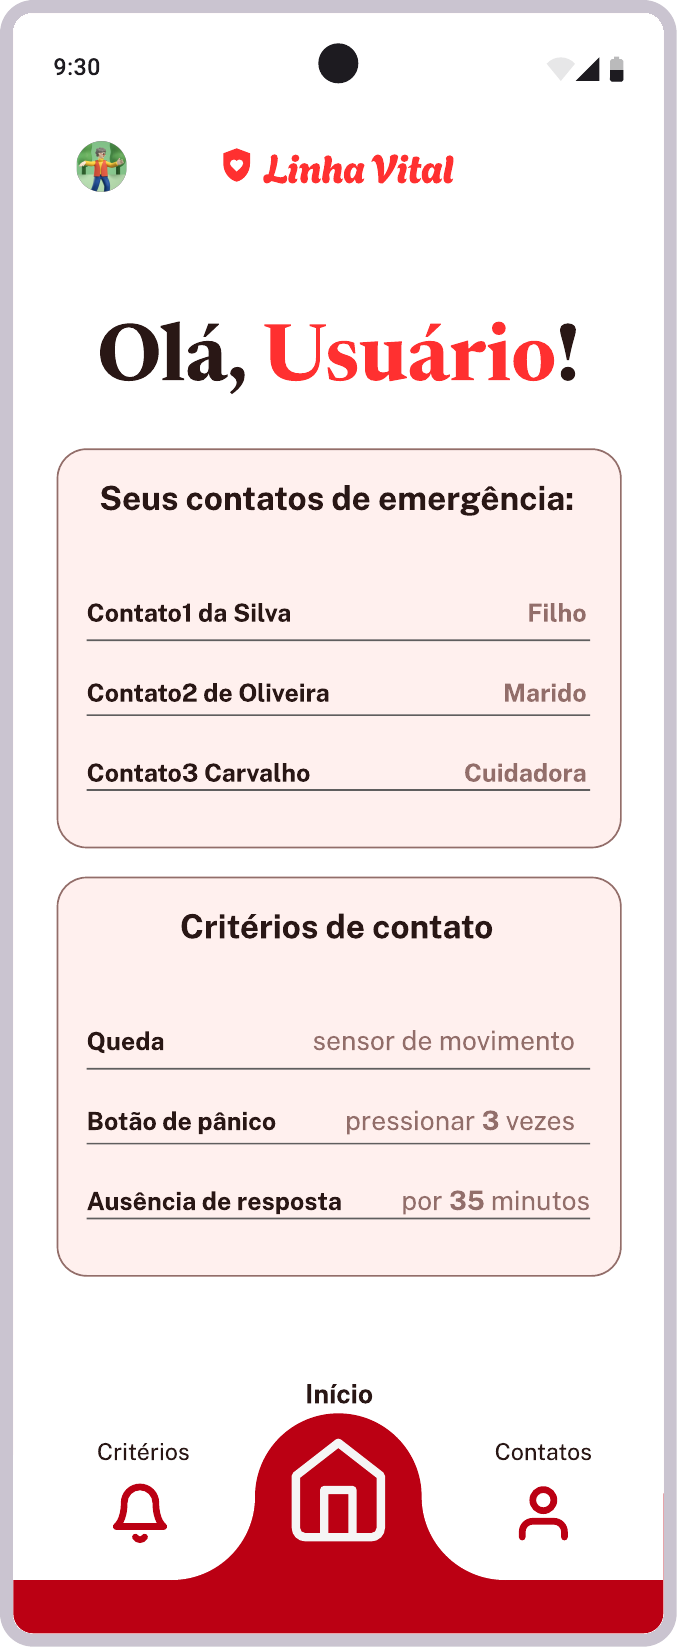
\includegraphics[width=0.32\textwidth]{imagens/prototipo_home.png}\caption{Protótipo da tela principal e estado do monitoramento.}\label{fig_proto_home}\legend{Fonte: Elaborado pelos autores.}\end{figure}
\begin{figure}[H]\centering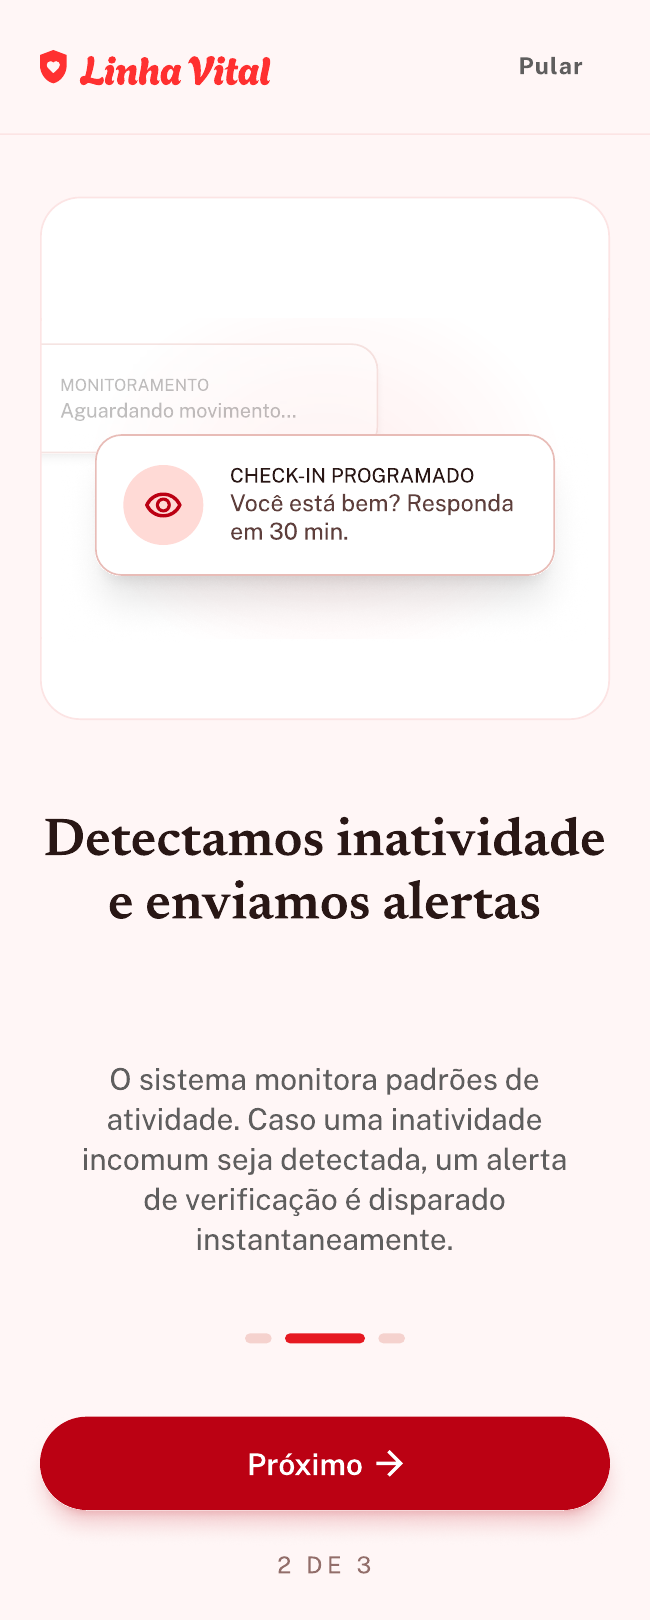
\includegraphics[width=0.32\textwidth]{imagens/prototipo_checkin.png}\caption{Protótipo da confirmação periódica de bem-estar.}\label{fig_proto_checkin}\legend{Fonte: Elaborado pelos autores.}\end{figure}
\begin{figure}[H]\centering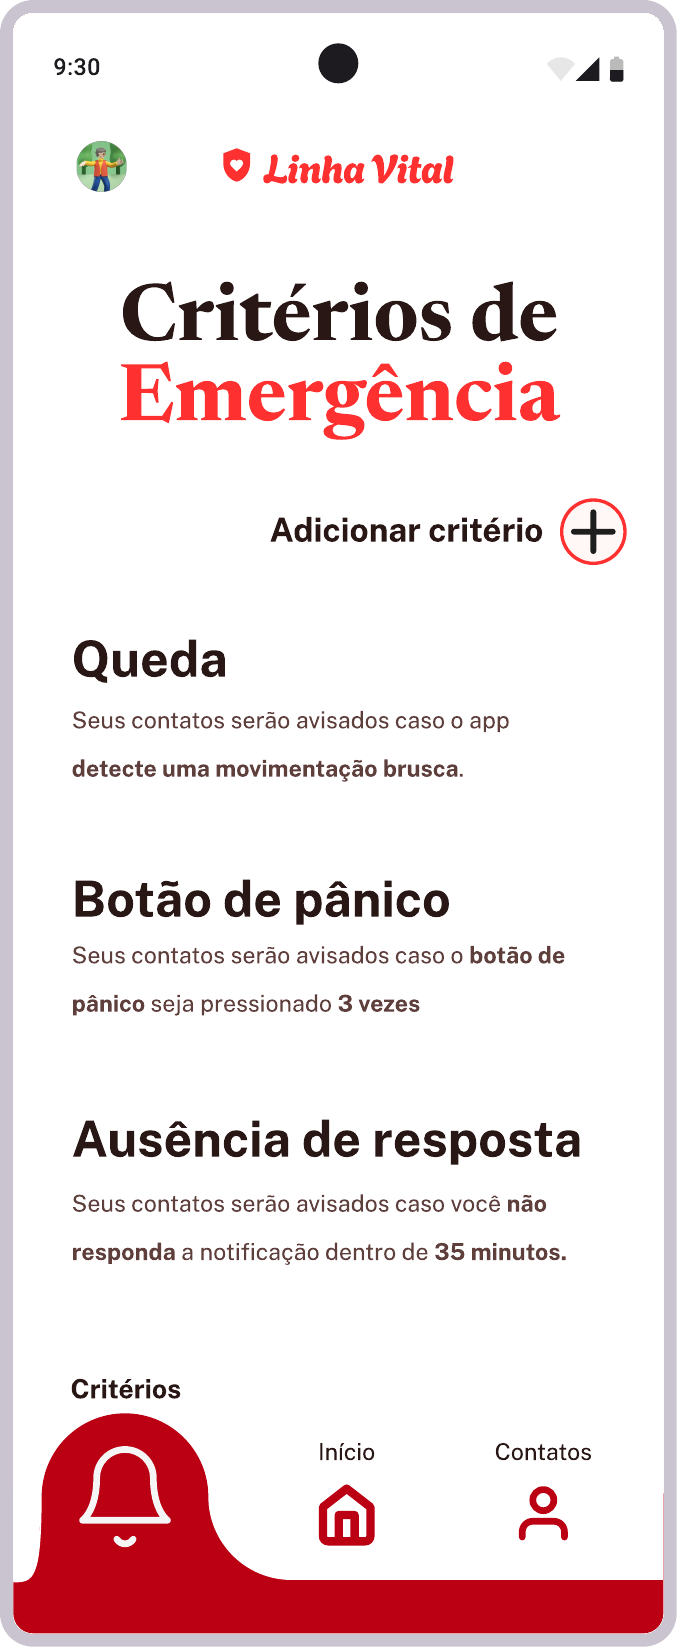
\includegraphics[width=0.32\textwidth]{imagens/prototipo_criterios.png}\caption{Proposta inicial da tela de critérios, com recursos não incluídos no MVP (por exemplo, detecção de quedas).}\label{fig_proto_criterios}\legend{Fonte: Elaborado pelos autores.}\end{figure}
\begin{figure}[H]\centering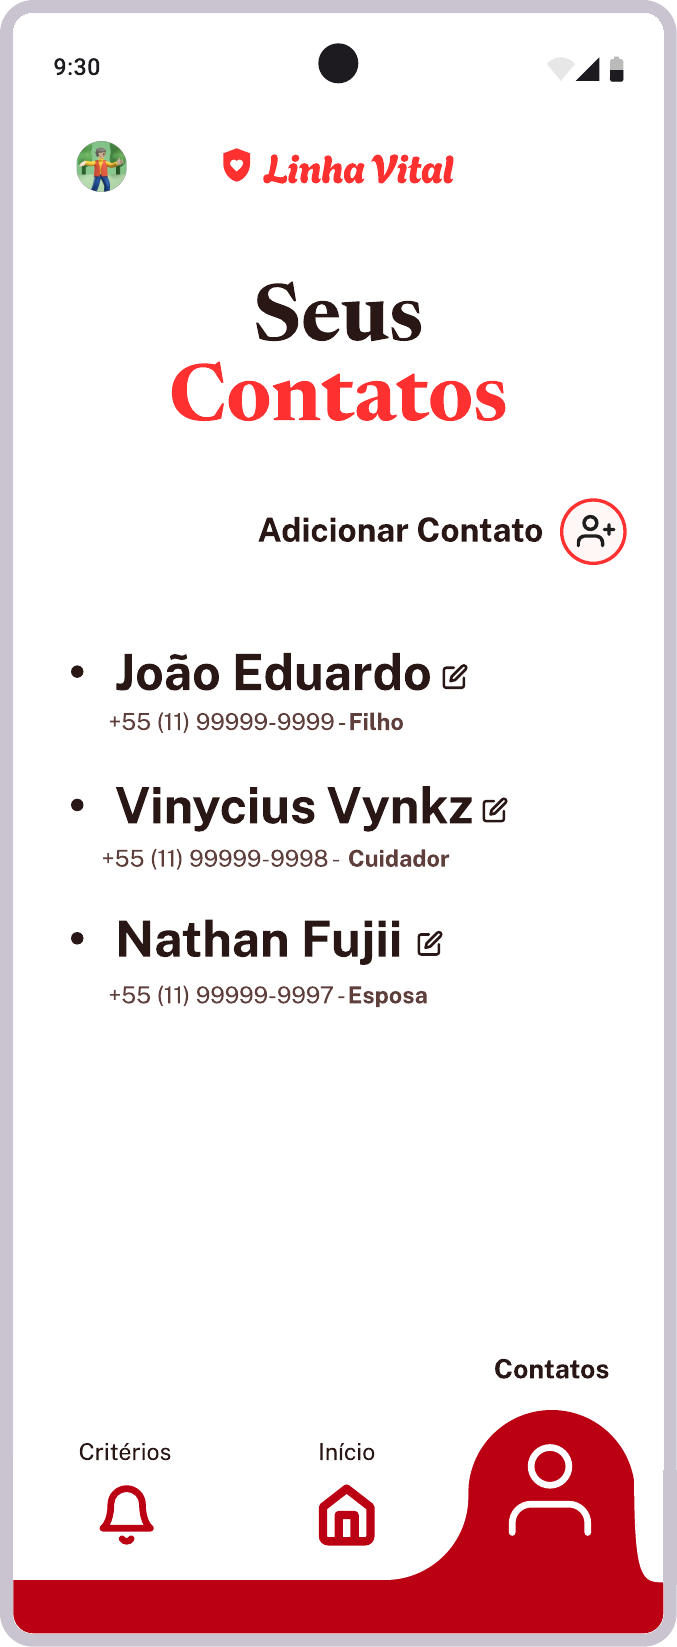
\includegraphics[width=0.32\textwidth]{imagens/prototipo_contatos.png}\caption{Protótipo da tela de gerenciamento de contatos.}\label{fig_proto_contatos}\legend{Fonte: Elaborado pelos autores.}\end{figure}


\subsection{Diferenças entre prototipação e versão entregue}

A imagem da tela de critérios representa uma proposta inicial com ideias, como detecção de quedas, que não foram implementadas. A evidência visual final deve ser capturada diretamente da versão Android executada, sem substituir protótipos por montagens. O Quadro~\ref{tab_proto_vs_mvp} delimita essas diferenças.

\begin{table}[H]
\caption{Concepção inicial versus entrega do MVP}
\label{tab_proto_vs_mvp}
\centering\footnotesize
\begin{tabular}{p{4cm}p{5cm}p{4cm}}\hline
\textbf{Funcionalidade} & \textbf{Versão entregue} & \textbf{Situação}
\\\hline
Check-in de bem-estar & Ação na Home e lembrete local & Implementado; sujeito a permissões \\\hline
Detecção de quedas & Não faz parte do monitoramento & Evolução futura \\\hline
Critério de inatividade & Intervalo de 1 a 240 minutos; tolerância no backend & Implementado com limitações \\\hline
SOS & Cascata assistida de ligações & Implementado com confirmação manual \\\hline
Localização & Captura sob demanda, com permissão & Não é rastreamento contínuo \\\hline
\end{tabular}
\legend{Fonte: Elaborado pelos autores, com base no código entregue.}
\end{table}

\noindent\textit{Evidências visuais disponíveis:} o relatório da bateria funcional de 14/10/2026 contém 111 capturas originais, identificadas de E001 a E111, abrangendo telas do emulador, consultas PostgreSQL e notificações. As figuras a seguir reproduzem exemplos selecionados do documento fornecido pela equipe, sem criar ou simular telas. Todas as imagens devem ser revisadas quanto a dados pessoais antes de divulgação pública.

\section{Testes e Manutenibilidade}

A etapa de testes funcionais da versão acadêmica foi concluída e documentada pela equipe. A apresentação dos resultados distingue o \textbf{planejamento original} da \textbf{bateria efetivamente executada}, evitando atribuir execução aos casos que aparecem apenas no plano.

\subsection{Plano de Testes}

O planejamento original contemplou testes unitários, verificações de integração da API com PostgreSQL e autenticação, testes de interface Android e cenários ponta a ponta para cadastro, login, check-in, inatividade, comunicação com contatos e SOS. Também previa medições não funcionais de latência, bateria, conectividade e carga. A bateria funcional efetivamente concluída e comprovada é descrita nas seções seguintes; as medições não documentadas não são apresentadas como resultados realizados.

A adoção de JUnit 5 está consolidada no backend. Bibliotecas de mocking, testes de integração com banco isolado e ferramentas de carga somente serão declaradas como parte da execução quando estiverem adicionadas ao projeto e utilizadas em resultados reproduzíveis.

\subsection{Metodologia e delimitação dos resultados}

A análise contempla duas fontes distintas: (i) os arquivos de testes automatizados identificados no código da versão entregue e (ii) o \emph{Relatório da Bateria de Testes e Evidências}, relativo à validação funcional pré-\textit{deploy} de \textbf{14 de outubro de 2026}. O segundo documento registra a execução de cenários integrados entre aplicativo Android, API Kotlin/Spring Boot e banco PostgreSQL, com resultados observados e capturas de evidências. A análise documental realizada em novembro não constitui nova execução dos testes; a aprovação relatada vale para o ambiente e a revisão de código utilizados no ensaio.

\subsubsection{Planejamento original versus execução registrada}

O documento \emph{Plano de Testes Linha Vital -- Reformulado}, de 04/09/2026, descreve \textbf{36 casos planejados} e propõe técnicas de partição de equivalência, valores-limite, cenários positivos e negativos, validação de contratos e integração, verificações de banco de dados e ensaios de interface, desempenho, segurança e confiabilidade. São considerados critérios de entrada: requisitos testáveis, versão identificada, ambiente disponível, dados preparados, dependências controladas e condições de aceite definidas. Como critérios de saída pretendidos, o plano registra conclusão dos casos críticos, inexistência de defeitos bloqueadores, regressão e registro de evidências e riscos residuais.

Para evitar ambiguidade, designam-se os casos do plano como \textbf{PL-CT01 a PL-CT36}, enquanto os \textbf{EX-CT01 a EX-CT17} (com EX-CT14A, B e C) identificam os 19 cenários da bateria executada em 14/10/2026. Os códigos usados originalmente nos dois documentos coincidem, mas \emph{não estabelecem equivalência automática entre os cenários}. Por exemplo, o caso planejado CT03 exige duas categorias distintas de contato, enquanto a versão implementada e o EX-CT03 verificam a presença de pelo menos um contato vinculado.

A equipe concluiu a bateria funcional registrada, que oferece evidências para os fluxos críticos descritos abaixo. O relatório, entretanto, \textbf{não demonstra a execução individual dos 36 casos previstos no plano original}, nem comprova metas quantitativas de desempenho, acessibilidade com usuários reais, segurança ofensiva ou alta disponibilidade. Não existe assinatura de aceite formal do parceiro anexada a esta versão.

\subsection{Ambiente e versão da bateria funcional}

Conforme o relatório da equipe, os testes utilizaram o \textbf{emulador Pixel 6 com Android API 33}, backend local em \textbf{Kotlin/Spring Boot 3.5.13 e Java 17}, porta 8080, acesso do emulador pelo endereço \texttt{10.0.2.2}, porta 8080, e persistência PostgreSQL consultada diretamente. A revisão consolidada no relatório é a branch \path{fix/correcoes-pre-testes}, após o \textit{merge} \texttt{0b7b01f}. O backend Oracle foi interrompido durante a validação local para impedir dois agendadores concorrentes sobre o mesmo banco. Essa condição é uma delimitação importante para a reprodutibilidade do ensaio.

\subsection{Resultados da bateria funcional pré-deploy}

A bateria funcional concluída pela equipe registra \textbf{19 cenários} (EX-CT01 a EX-CT17, com EX-CT14 subdividido em A, B e C; na coluna ID da tabela, o prefixo EX- é omitido para facilitar a leitura): \textbf{17 aprovados} e \textbf{2 aprovados com observações} (CT14B e CT15). Os resultados correspondem à classificação original dos executores, não a uma auditoria independente de funcionamento em produção. As evidências são identificadas pelos códigos \texttt{E001--E111} no Apêndice A do relatório de testes, preservado integralmente no repositório revisado, em \emph{Documentacao/Evidencias/}.

\begingroup
\footnotesize
\renewcommand{\arraystretch}{1.12}
\begin{longtable}{p{1.0cm}p{3.3cm}p{4.3cm}p{2.0cm}p{2.1cm}}
\caption{Matriz de cenários da bateria de testes de 14/10/2026}\label{tab_validacao_integrada}\\
\hline
\textbf{ID} & \textbf{Cenário} & \textbf{Resultado observado} & \textbf{Situação} & \textbf{Evidências}\\\hline
\endfirsthead
\multicolumn{5}{l}{\footnotesize Continuação da matriz de testes funcionais}\\\hline
\textbf{ID} & \textbf{Cenário} & \textbf{Resultado observado} & \textbf{Situação} & \textbf{Evidências}\\\hline
\endhead
CT01 & Conexão com backend local & API acessível pelo emulador & Aprovado & E002\\\hline
CT02 & Usuário inicial pausado & Home indica monitoramento pausado & Aprovado & E005, E093\\\hline
CT03 & Ativação sem contato & Ativação recusada na branch consolidada & Aprovado & E096\\\hline
CT04 & Contatos e prioridades & Vínculos e prioridades 1 e 2 no banco & Aprovado & E030, E097\\\hline
CT05 & Notificação de check-in & Notificação exibida; toque reabre o aplicativo & Aprovado & E010, E054\\\hline
CT06 & Inatividade e e-mail & Alerta e registro ENVIADO; e-mail recebido no ensaio & Aprovado & E014, E065, E066\\\hline
CT07 & Confirmação ``Estou bem'' & Inatividade resolvida; ciclo reiniciado & Aprovado & E018, E103, E104\\\hline
CT08 & SOS básico & PANICO resolvido após ATENDIDO & Aprovado & E028, E029\\\hline
CT09 & Cascata por prioridade & NAO\_ATENDIDO avança; ATENDIDO encerra & Aprovado & E031, E032, E106\\\hline
CT10 & Exclusão com histórico & Vínculo removido; histórico preservado & Aprovado & E038--E040\\\hline
CT11 & Exclusão sem histórico & Vínculo e registro do contato removidos & Aprovado & E044--E046\\\hline
CT12 & Edição de contato & ID e prioridade mantidos; dados novos usados & Aprovado & E047, E048, E051, E053\\\hline
CT13 & Aplicativo fechado/force-stop & Backend permaneceu monitorando; sessão persistiu & Aprovado & E054, E068--E070\\\hline
CT14A & Localização negada & Check-in continua; localização não gravada & Aprovado & E073, E074, E076, E077\\\hline
CT14B & Ligação negada & Sem travamento; PANICO ativo; TENTATIVA registrada & Aprovado com obs. & E078--E081\\\hline
CT14C & Notificação negada & Sem notificação local; backend e e-mails mantidos & Aprovado & E082--E085\\\hline
CT15 & Backend indisponível & Falhas tratadas; recuperação e SOS resolvido & Aprovado com obs. & E086, E087, E089, E091, E092\\\hline
CT16 & Regressão ponta a ponta & Novo usuário percorreu os fluxos principais & Aprovado & E093, E096, E097, E101, E102, E105, E110\\\hline
CT17 & Logout/login & Monitoramento pausado; dados recuperados & Aprovado & E107, E110, E111\\\hline
\end{longtable}
\endgroup
\noindent\footnotesize\textit{Fonte:} Relatório da Bateria de Testes e Evidências, 14/10/2026, seção 4, pp. 4 e 8--35. Os códigos de evidência remetem ao apêndice do próprio relatório.\normalsize

\subsubsection{Fluxos validados e evidências selecionadas}

\textbf{Monitoramento e inatividade:} o usuário novo iniciou com o monitoramento pausado; a ativação sem contato foi impedida na versão consolidada. Com contato cadastrado e intervalo reduzido para 1 minuto para fins de teste, foram observados lembrete de check-in, geração de alerta de inatividade, registro de envio por contato e recebimento de e-mail no cenário ensaiado. O botão ``Estou bem'' encerrou o alerta e reiniciou o ciclo (CT02--CT07).

\begin{figure}[H]
\centering
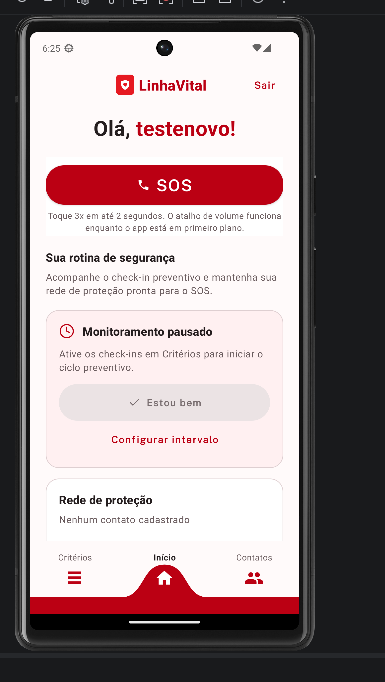
\includegraphics[height=5.2cm,keepaspectratio]{imagens/e005_estado_inicial.png}\hspace{1.0cm}
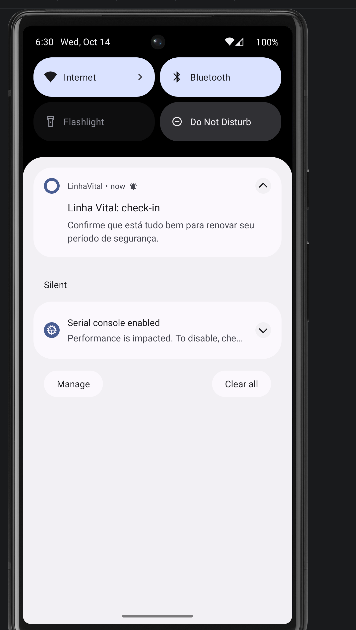
\includegraphics[height=5.2cm,keepaspectratio]{imagens/e010_notificacao_local.png}
\caption{Evidências de monitoramento inicial e lembrete local: E005 e E010 (14/10/2026).}
\legend{Fonte: Relatório da Bateria de Testes e Evidências, Apêndice A, pp. 9--10.}
\end{figure}

\textbf{SOS e contatos:} o SOS criado após três interações utilizou contatos ordenados por prioridade. O registro NAO\_ATENDIDO levou à próxima tentativa; o registro ATENDIDO permitiu resolver o alerta PANICO. A exclusão de contato com histórico preservou a referência histórica, enquanto a exclusão sem histórico removeu os registros associados ao teste; a edição manteve identidade e prioridade do contato (CT08--CT12).

\textbf{Permissões, resiliência e regressão:} foram testadas a continuidade do monitoramento no backend com o aplicativo fechado ou em \textit{force-stop}, as permissões de localização, ligação e notificação negadas, a indisponibilidade temporária do backend e a recuperação após seu retorno. A regressão final percorreu cadastro, contatos, inatividade, e-mail, SOS, exclusão, logout e novo login (CT13--CT17). O resultado não deve ser interpretado como garantia de notificações locais após \textit{force-stop}, já que a evidência específica confirma a persistência do monitoramento no servidor.

\begin{figure}[H]
\centering
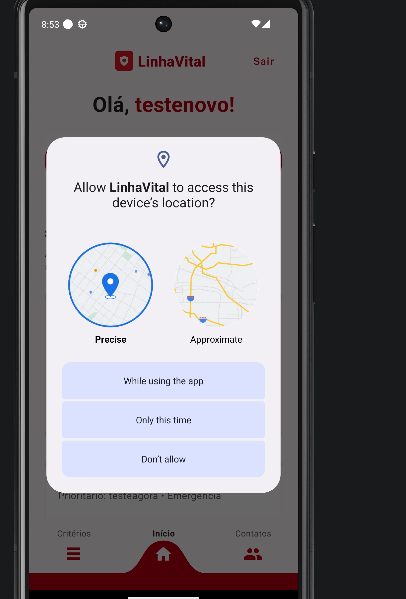
\includegraphics[height=5.2cm,keepaspectratio]{imagens/e073_permissao_localizacao.png}\hspace{1.0cm}
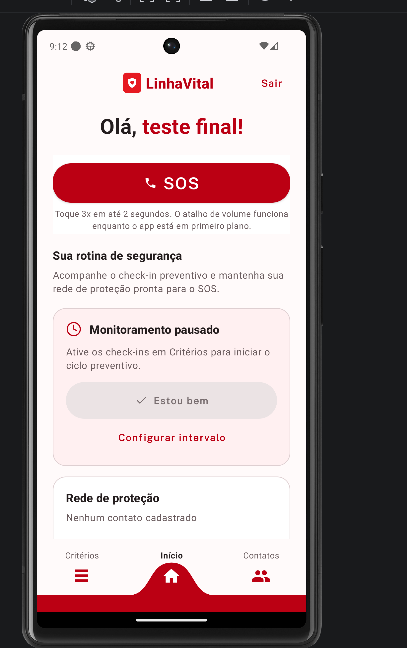
\includegraphics[height=5.2cm,keepaspectratio]{imagens/e093_regressao_usuario_novo.png}
\caption{Evidências de tratamento de permissão e regressão final: E073 e E093 (14/10/2026).}
\legend{Fonte: Relatório da Bateria de Testes e Evidências, Apêndice A, pp. 26 e 31.}
\end{figure}

\subsubsection{Incidentes resolvidos e observações não bloqueantes}

O documento registra dois incidentes de ambiente: (i) alertas duplicados quando o backend local e uma instância Oracle executavam o agendador simultaneamente sobre o mesmo banco, corrigidos com a interrupção da segunda instância; e (ii) execução inicial de uma branch desatualizada, que permitia ativação sem contato, corrigida ao utilizar \texttt{fix/correcoes-pre-testes}. Tais ocorrências foram tratadas e o cenário foi repetido no ambiente consolidado. Persistem observações de experiência de uso: mensagem técnica de conexão na tela de contatos quando a API está indisponível; redação potencialmente ambígua da mensagem de continuidade do SOS nessa condição; e falta de um status específico para ligação bloqueada por permissão. Essas limitações não foram apagadas da apresentação dos resultados.

\subsection{Inventário de testes automatizados versionados}

A inspeção estática do código em 12/11/2026 identificou classes de testes Kotlin para monitoramento, cadastro, senhas, datas e interações de SOS. Seu inventário é separado da bateria manual, pois o relatório funcional de outubro não é um relatório de execução JUnit, nem registra percentual de cobertura.

\begin{table}[H]
\caption{Inventário dos testes automatizados presentes no código}
\label{tab_resultados_testes}
\centering\footnotesize
\renewcommand{\arraystretch}{1.15}
\begin{tabular}{p{4.3cm}p{8.6cm}}\hline
\textbf{Classe e quantidade} & \textbf{Cenários cobertos no código}\\\hline
\texttt{PasswordServiceTests} (2) & Hash, verificação e migração de senha\\\hline
\texttt{UsuarioServiceTests} (5) & Validação de campos cadastrais\\\hline
\texttt{MonitoramentoService} \texttt{Tests} (8) & Contato mínimo, tolerância, pausa, deduplicação e check-in\\\hline
\texttt{DataNascimentoUtils} \texttt{Test} (8) & Data inválida, ano bissexto e conversões\\\hline
\texttt{SosInteractionTracker} \texttt{Test} (7) & Contagem e janela de interações do SOS\\\hline
\texttt{BackendApplication} \texttt{Tests} e exemplos Android & Contexto Spring e exemplos sem cobertura dos fluxos críticos\\\hline
\end{tabular}
\legend{Fonte: Inspeção dos arquivos de teste Kotlin do repositório, em 12/11/2026. Quantidades representam métodos localizados, não execuções.}
\end{table}

A etapa de documentação realizada em novembro não correspondeu a uma nova execução de testes JUnit/Android ou de verificações em ambiente de produção. A bateria funcional realizada em 14/10/2026 foi concluída e registra os \textit{resultados observados pela equipe} nos cenários exercitados naquela versão; não substitui ensaios formais de consumo de bateria, carga, latência, disponibilidade prolongada, segurança e acessibilidade. O relatório registra \texttt{BUILD SUCCESSFUL} após o merge da branch de testes, mas não apresenta um log completo e auditável da suíte automatizada.

\subsection{Análise Estática e Manutenibilidade}

A análise estática e as convenções de código são utilizadas como mecanismos complementares para identificar inconsistências, problemas de manutenção e riscos de segurança. A evolução desse processo deve incluir execução automatizada de lint, verificações de dependências e integração contínua, mantendo os resultados associados a uma versão específica do código.

\subsection{Logs}

O sistema deverá registrar eventos relevantes relacionados ao funcionamento da aplicação, incluindo operações executadas, falhas de comunicação, erros de processamento e acionamentos de emergência. Esses registros contribuirão para atividades de monitoramento, manutenção e diagnóstico de problemas.

\subsection{Code Convention}

O desenvolvimento do sistema seguirá padrões de codificação compatíveis com as boas práticas recomendadas para projetos Kotlin e Spring Boot. A adoção dessas convenções tem como objetivo promover maior legibilidade, padronização, manutenibilidade e organização do código-fonte, facilitando o trabalho colaborativo da equipe de desenvolvimento.

\section{Segurança, Privacidade e Legislação}

Considerando que o sistema Linha Vital realiza o armazenamento e processamento de informações pessoais, contatos emergenciais e registros de monitoramento comportamental, foram definidos critérios voltados à proteção de dados, segurança da informação e conformidade legal.

A aplicação foi projetada visando reduzir riscos relacionados a acesso indevido, vazamento de informações, uso inadequado de dados pessoais e falhas de autenticação, buscando preservar a privacidade e a integridade das informações dos usuários.

\subsection{Critérios de Segurança e Privacidade}

O sistema adota mecanismos de autenticação e controle de acesso com o objetivo de restringir a utilização da aplicação apenas a usuários autorizados. Senhas recebem derivação PBKDF2 com salt e sessões empregam tokens Bearer opacos cujos hashes são persistidos no backend; esses controles reduzem riscos específicos sem eliminá-los.

No aplicativo Android, a configuração de segurança de rede proíbe tráfego HTTP por padrão, mas contém exceções explícitas para o emulador/ambiente local e para o endereço de homologação da máquina virtual. Portanto, não é correto afirmar que todo tráfego está protegido por HTTPS nesta versão. Antes de implantação pública, as exceções de texto claro devem ser removidas e a API disponibilizada sobre TLS com validação adequada de certificados. Há validações de entrada e autorização por recurso em componentes do backend, ainda sujeitas a auditoria sistemática.

A arquitetura da aplicação foi organizada em camadas separadas entre front-end, back-end e banco de dados, favorecendo maior controle estrutural, facilidade de manutenção e segurança operacional. Também são considerados mecanismos de controle de sessão, monitoramento de falhas e registro de eventos críticos para identificação de comportamentos anormais no sistema.

O projeto busca minimizar a coleta; contudo, cadastro, contatos, localização e logs devem passar por análise de finalidade, retenção, acesso e exclusão antes do uso público. Além disso, considera práticas voltadas à proteção de credenciais, tokens e variáveis sensíveis, reduzindo riscos de exposição inadequada durante o desenvolvimento e a implantação da solução.

Como mecanismo complementar de segurança, podem ser utilizadas ferramentas de análise estática de código (SAST), permitindo identificar vulnerabilidades, falhas de implementação e possíveis riscos de segurança ainda durante o processo de desenvolvimento.

\subsection{Observância à Legislação}

O desenvolvimento do sistema Linha Vital considera as diretrizes estabelecidas pela Lei Geral de Proteção de Dados Pessoais (LGPD), instituída pela Lei nº 13.709/2018, responsável por regulamentar o tratamento de dados pessoais no Brasil. Dessa forma, a aplicação busca limitar o tratamento às finalidades da aplicação, sem que esta revisão documental comprove conformidade jurídica integral.

A aplicação permite atualização cadastral e gerenciamento de contatos; ainda é necessária a formalização de política de privacidade, bases legais, retenção, tratamento de dados dos contatos e procedimentos de atendimento aos direitos dos titulares. Além disso, foram considerados mecanismos para reduzir riscos de acesso indevido, vazamento ou utilização inadequada das informações processadas pela plataforma.

A ISO/IEC 27001 é uma referência de gestão de segurança aplicável como orientação; o Linha Vital não passou por certificação nem auditoria de conformidade com essa norma. Essas práticas auxiliam na definição de controles voltados à proteção de dados, gerenciamento de acessos, mitigação de riscos computacionais e preservação da integridade das informações armazenadas pelo sistema.

Considerando que o Linha Vital pode lidar com situações críticas e dados relacionados ao bem-estar dos usuários, o projeto também observa princípios éticos ligados à privacidade, responsabilidade no tratamento das informações e utilização consciente dos recursos tecnológicos desenvolvidos.

\section{Modelo de Banco de Dados}

O modelo de dados foi atualizado a partir das dez classes JPA do pacote de modelos do backend. As figuras descrevem o mapeamento objeto-relacional encontrado no repositório em 12/11/2026. A estrutura física de um banco específico pode apresentar diferenças decorrentes de migrações e configurações do Hibernate; portanto, a validação final do esquema físico exige confronto com o banco implantado.

A Figura~\ref{fig_mer} apresenta a visão conceitual das entidades e das associações. A notação \texttt{N:1} significa vários registros da entidade de origem para um de destino; \texttt{1:1} representa vínculo único de configuração por usuário.

\begin{figure}[H]
\caption{Modelo de entidades do MVP baseado nas classes JPA.}
\label{fig_mer}
\centering
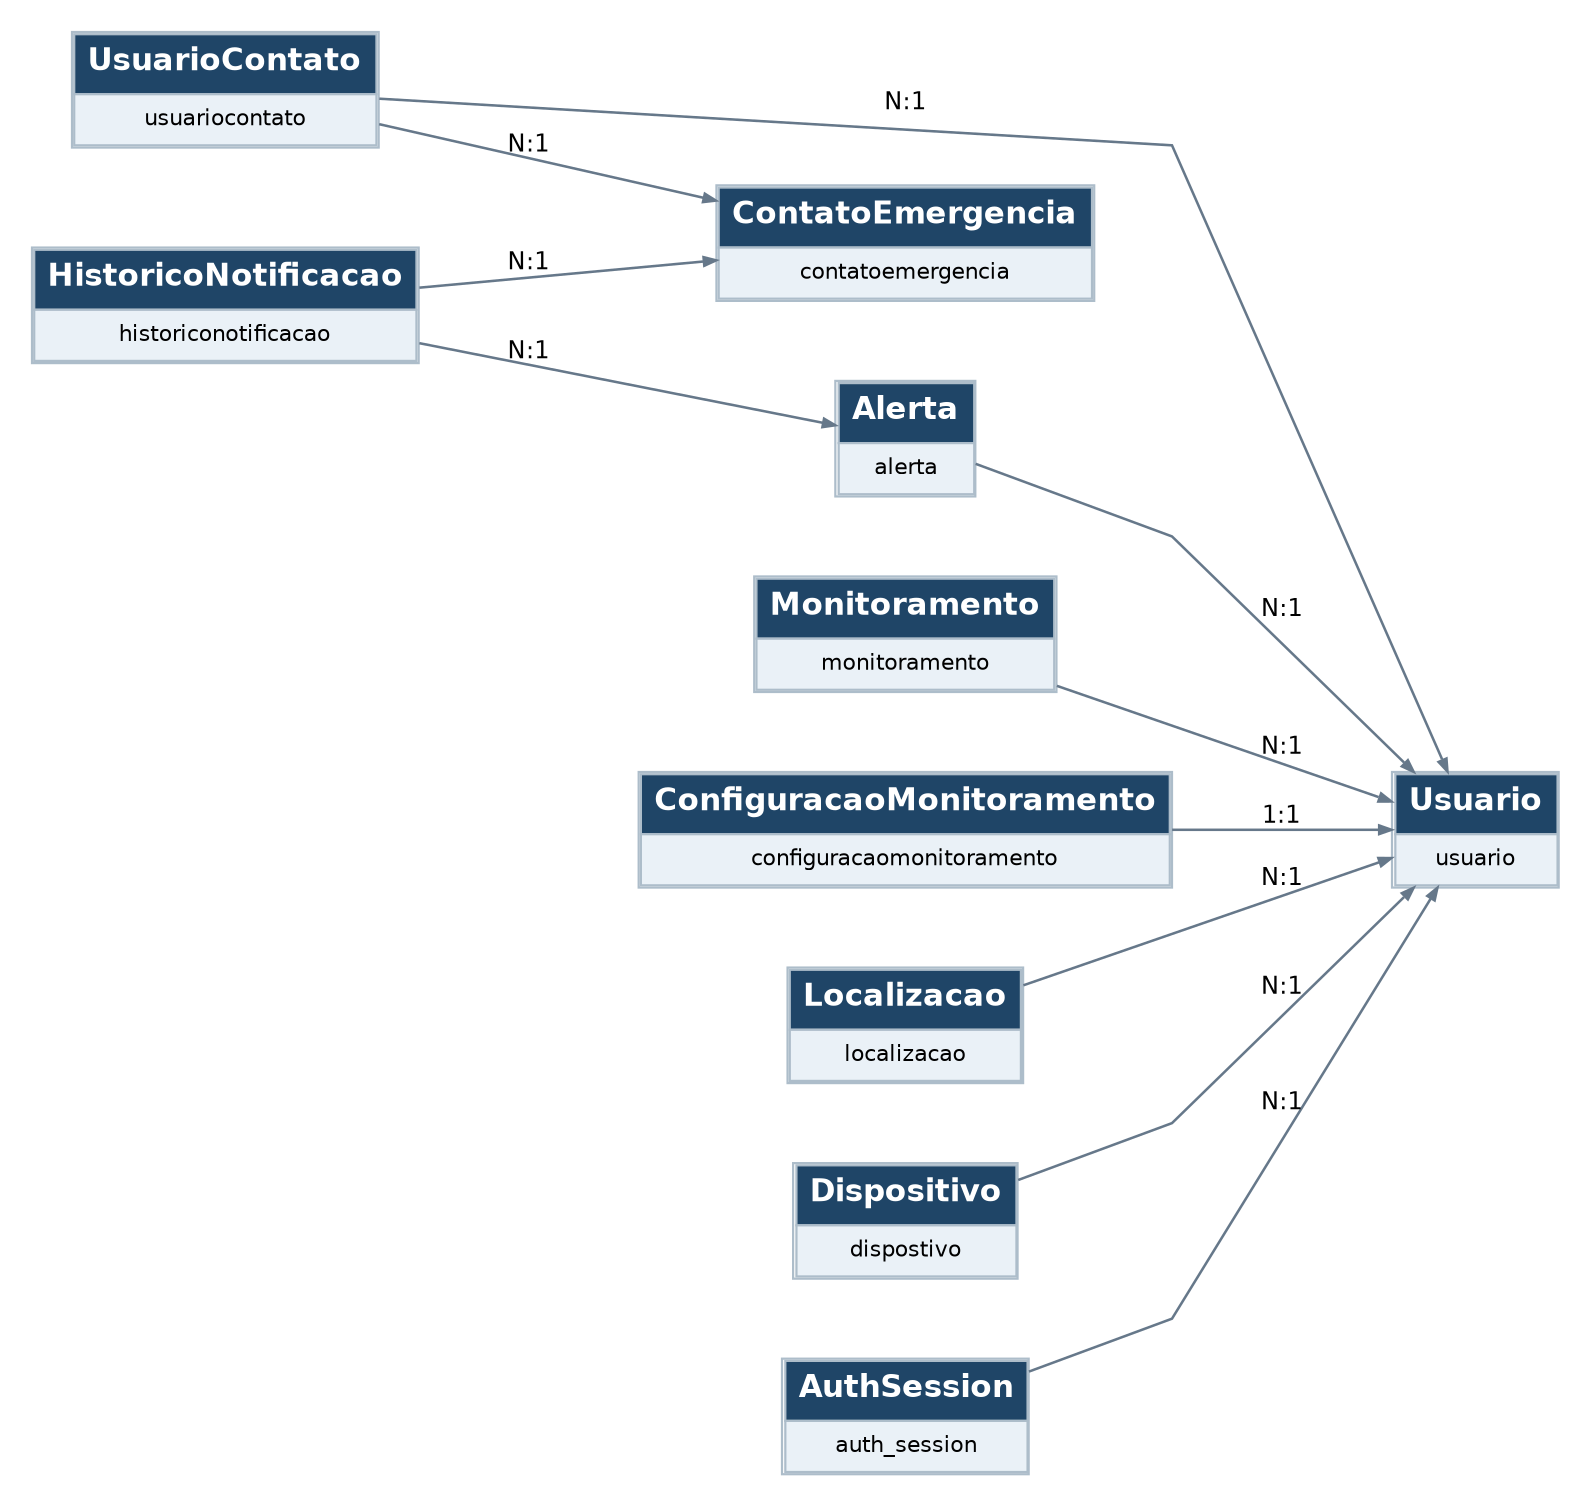
\includegraphics[width=\textwidth,height=0.72\textheight,keepaspectratio]{imagens/mer_jpa_2026.png}
\legend{Fonte: Elaborado pelos autores a partir do mapeamento JPA.}
\end{figure}

A Figura~\ref{fig_der} acrescenta os atributos e os tipos indicativos extraídos das entidades. A nomenclatura das tabelas e colunas preserva inclusive grafias legadas presentes em \texttt{@Table} e \texttt{@Column}, como \texttt{dispostivo} e \texttt{sistema\_dispositio}. Alterar esses nomes no banco sem migração coordenada poderia comprometer a aplicação.

\begin{figure}[H]
\caption{Diagrama lógico de entidades e atributos mapeados no backend.}
\label{fig_der}
\centering
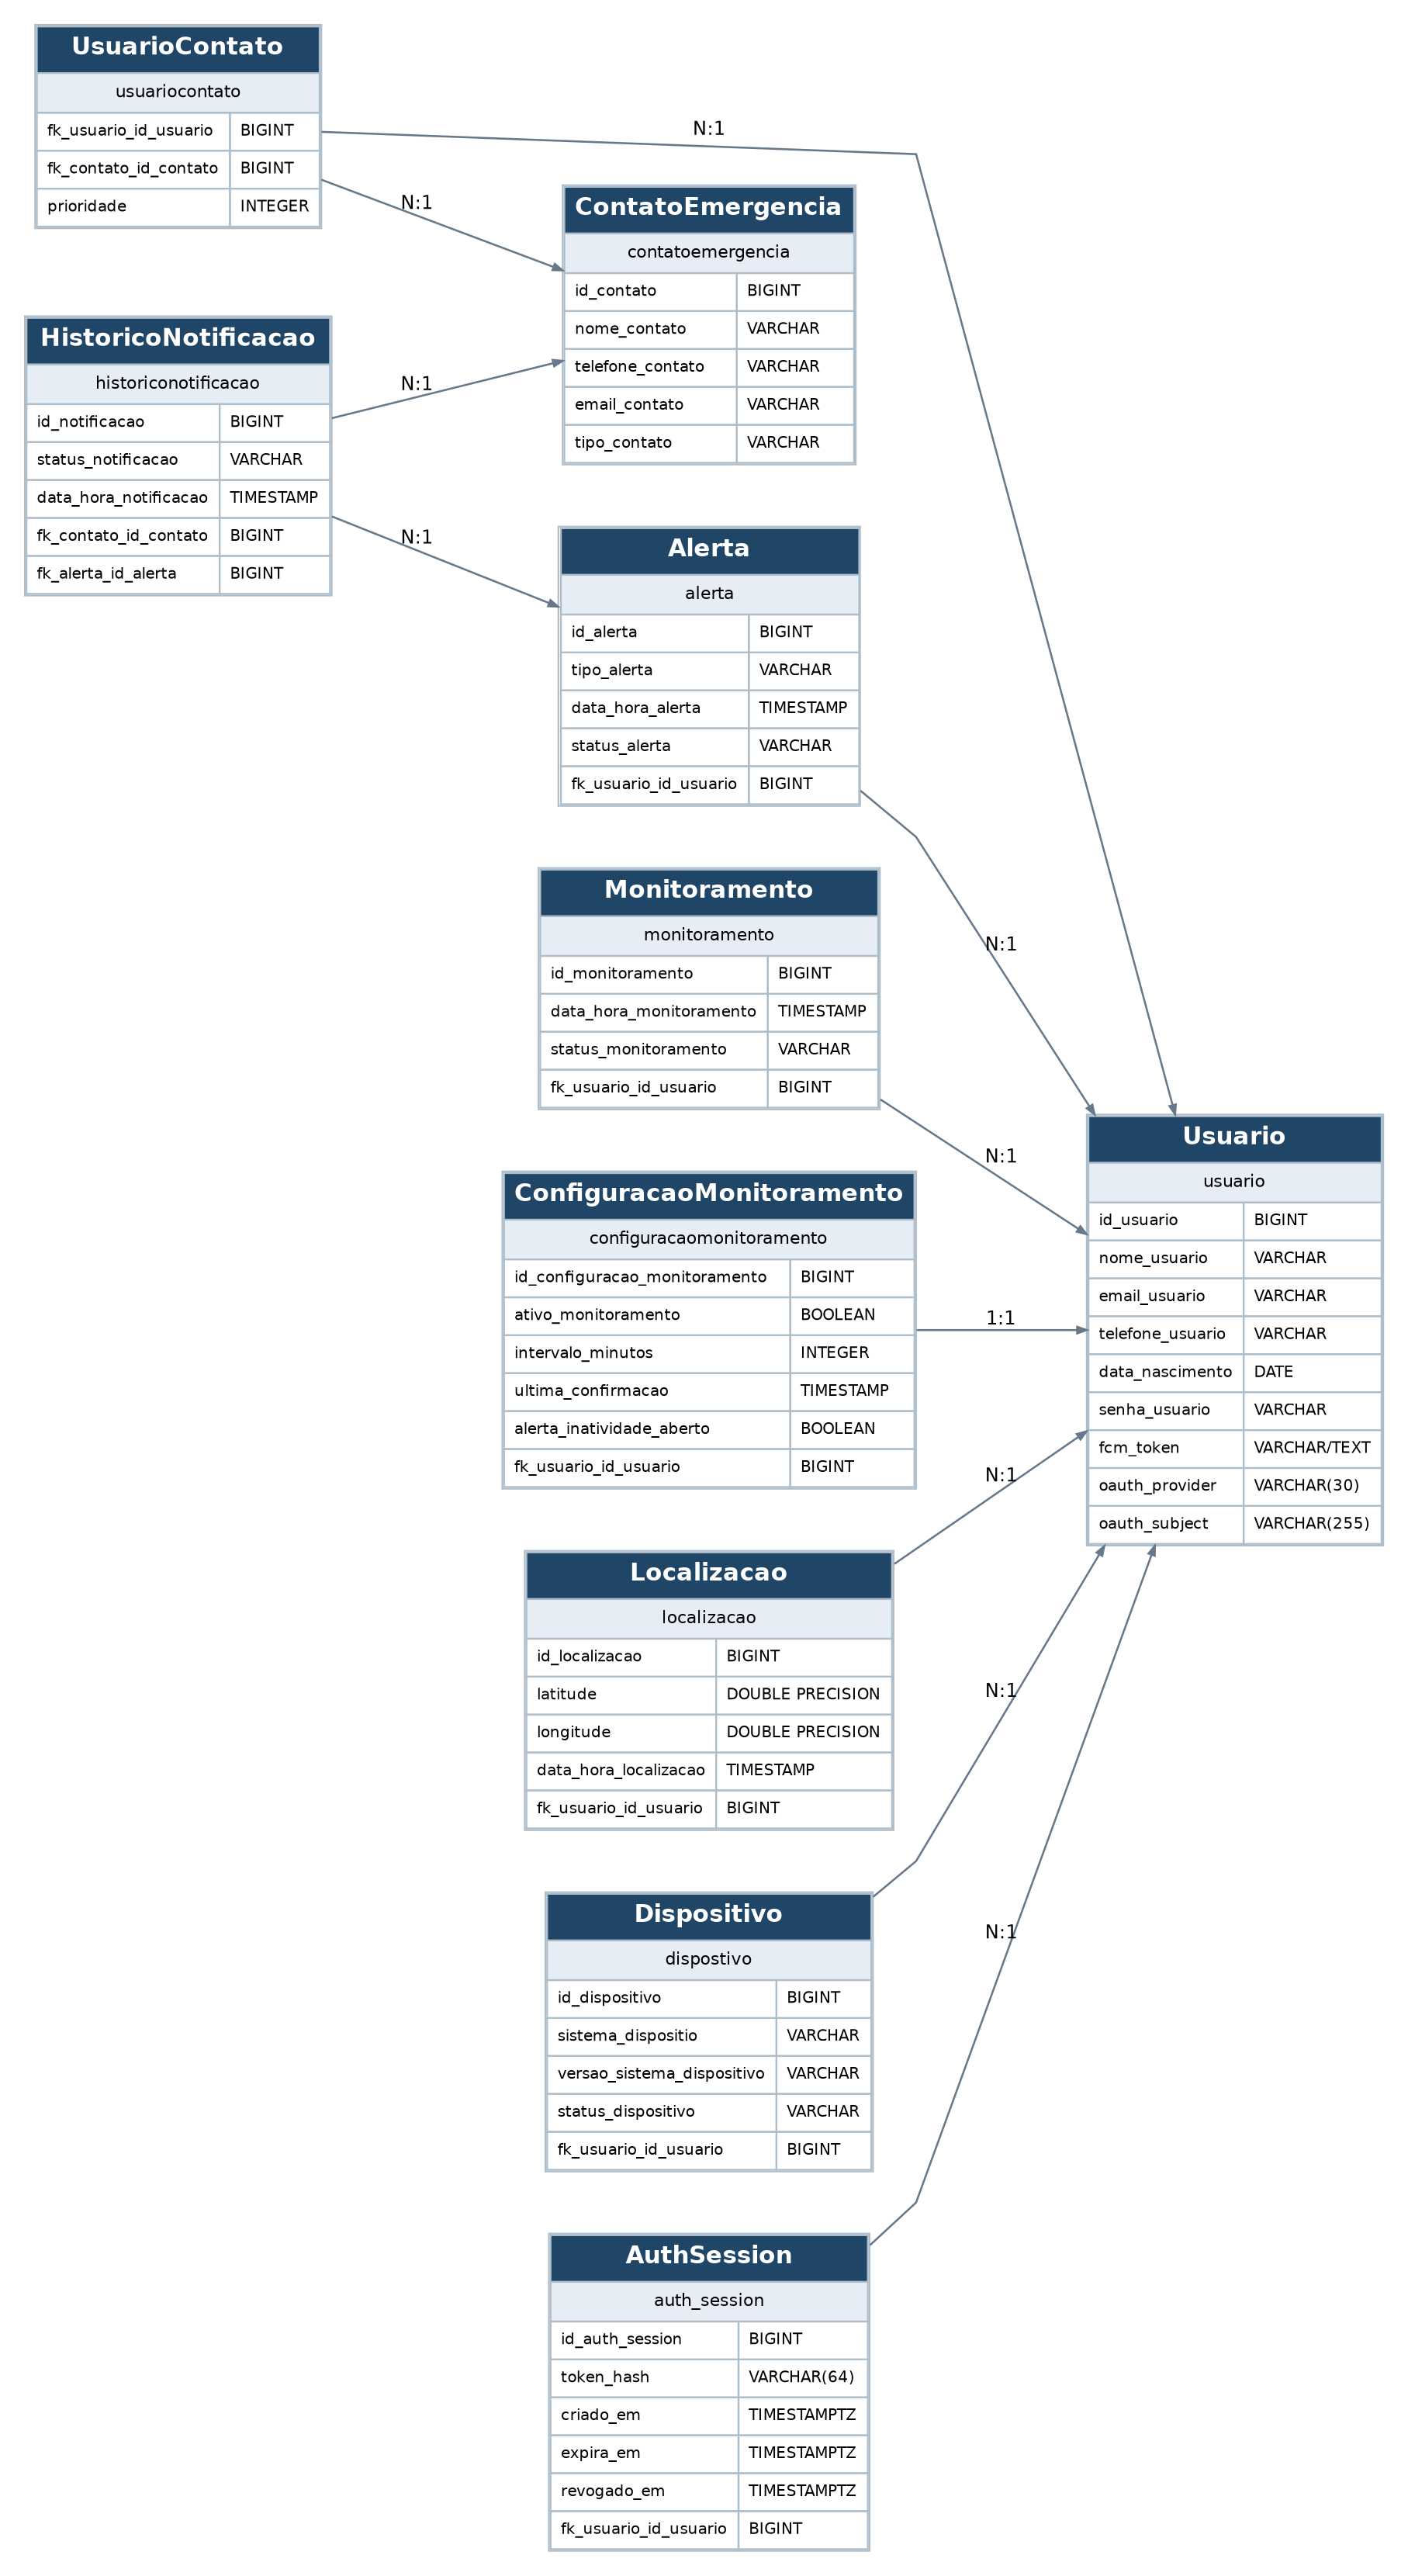
\includegraphics[width=\textwidth,height=0.79\textheight,keepaspectratio]{imagens/der_jpa_2026.png}
\legend{Fonte: Elaborado pelos autores a partir das classes JPA; tipos indicativos.}
\end{figure}

\subsection{Dicionário de Dados}

As dez entidades persistentes estão documentadas abaixo. Os tipos indicados são aproximações para PostgreSQL inferidas das propriedades Kotlin e anotações JPA, e não a transcrição de um script DDL do ambiente implantado. Colunas sem \texttt{nullable=false} explícito não devem ser automaticamente assumidas como obrigatórias; restrições adicionais podem resultar da geração do esquema, validações da aplicação ou migrações. PK significa chave primária e FK significa chave estrangeira.

\subsubsection{Entidade Usuario (\texttt{usuario})}

\begin{longtable}{p{4.8cm}p{3.05cm}p{5.05cm}}
\caption{Dicionário da entidade Usuario}\label{quad_usuario}\\
\hline
\textbf{Coluna} & \textbf{Tipo indicativo} & \textbf{Significado / restrição mapeada} \\
\hline
\endfirsthead
\hline\textbf{Coluna} & \textbf{Tipo indicativo} & \textbf{Significado / restrição mapeada} \\
\hline
\endhead
id\_usuario & BIGINT & PK, geração por identidade \\
\hline
nome\_usuario & VARCHAR & não nulo \\
\hline
email\_usuario & VARCHAR & não nulo, único \\
\hline
telefone\_usuario & VARCHAR & não nulo \\
\hline
data\_nascimento & DATE & não nulo \\
\hline
senha\_usuario & VARCHAR & não nulo; derivação PBKDF2 \\
\hline
fcm\_token & VARCHAR/TEXT & opcional \\
\hline
oauth\_provider & VARCHAR(30) & opcional \\
\hline
oauth\_subject & VARCHAR(255) & opcional; único com provider \\
\hline
\end{longtable}

\subsubsection{Entidade ContatoEmergencia (\texttt{contatoemergencia})}

\begin{longtable}{p{4.8cm}p{3.05cm}p{5.05cm}}
\caption{Dicionário da entidade ContatoEmergencia}\label{quad_contato}\\
\hline
\textbf{Coluna} & \textbf{Tipo indicativo} & \textbf{Significado / restrição mapeada} \\
\hline
\endfirsthead
\hline\textbf{Coluna} & \textbf{Tipo indicativo} & \textbf{Significado / restrição mapeada} \\
\hline
\endhead
id\_contato & BIGINT & PK, identidade \\
\hline
nome\_contato & VARCHAR & nome \\
\hline
telefone\_contato & VARCHAR & telefone \\
\hline
email\_contato & VARCHAR & e-mail \\
\hline
tipo\_contato & VARCHAR & categoria \\
\hline
\end{longtable}

\subsubsection{Entidade UsuarioContato (\texttt{usuariocontato})}

\begin{longtable}{p{4.8cm}p{3.05cm}p{5.05cm}}
\caption{Dicionário da entidade UsuarioContato}\label{quad_usuario_contato}\\
\hline
\textbf{Coluna} & \textbf{Tipo indicativo} & \textbf{Significado / restrição mapeada} \\
\hline
\endfirsthead
\hline\textbf{Coluna} & \textbf{Tipo indicativo} & \textbf{Significado / restrição mapeada} \\
\hline
\endhead
fk\_usuario\_id\_usuario & BIGINT & PK composta e FK Usuario \\
\hline
fk\_contato\_id\_contato & BIGINT & PK composta e FK ContatoEmergencia \\
\hline
prioridade & INTEGER & prioridade do vínculo \\
\hline
\end{longtable}

\subsubsection{Entidade Monitoramento (\texttt{monitoramento})}

\begin{longtable}{p{4.8cm}p{3.05cm}p{5.05cm}}
\caption{Dicionário da entidade Monitoramento}\label{quad_monitoramento}\\
\hline
\textbf{Coluna} & \textbf{Tipo indicativo} & \textbf{Significado / restrição mapeada} \\
\hline
\endfirsthead
\hline\textbf{Coluna} & \textbf{Tipo indicativo} & \textbf{Significado / restrição mapeada} \\
\hline
\endhead
id\_monitoramento & BIGINT & PK, identidade \\
\hline
data\_hora\_monitoramento & TIMESTAMP & registro do evento \\
\hline
status\_monitoramento & VARCHAR & estado registrado \\
\hline
fk\_usuario\_id\_usuario & BIGINT & FK Usuario \\
\hline
\end{longtable}

\subsubsection{Entidade ConfiguracaoMonitoramento (\texttt{configuracaomonitoramento})}

\begin{longtable}{p{4.8cm}p{3.05cm}p{5.05cm}}
\caption{Dicionário da entidade ConfiguracaoMonitoramento}\label{quad_configuracaomonitoramento}\\
\hline
\textbf{Coluna} & \textbf{Tipo indicativo} & \textbf{Significado / restrição mapeada} \\
\hline
\endfirsthead
\hline\textbf{Coluna} & \textbf{Tipo indicativo} & \textbf{Significado / restrição mapeada} \\
\hline
\endhead
id\_configuracao\_monitoramento & BIGINT & PK, identidade \\
\hline
ativo\_monitoramento & BOOLEAN & não nulo; ativação \\
\hline
intervalo\_minutos & INTEGER & não nulo; 1 a 240 na API \\
\hline
ultima\_confirmacao & TIMESTAMP & não nulo; check-in \\
\hline
alerta\_inatividade\_aberto & BOOLEAN & não nulo; controle de duplicação \\
\hline
fk\_usuario\_id\_usuario & BIGINT & FK Usuario; único, não nulo \\
\hline
\end{longtable}

\subsubsection{Entidade Alerta (\texttt{alerta})}

\begin{longtable}{p{4.8cm}p{3.05cm}p{5.05cm}}
\caption{Dicionário da entidade Alerta}\label{quad_alerta}\\
\hline
\textbf{Coluna} & \textbf{Tipo indicativo} & \textbf{Significado / restrição mapeada} \\
\hline
\endfirsthead
\hline\textbf{Coluna} & \textbf{Tipo indicativo} & \textbf{Significado / restrição mapeada} \\
\hline
\endhead
id\_alerta & BIGINT & PK, identidade \\
\hline
tipo\_alerta & VARCHAR & categoria \\
\hline
data\_hora\_alerta & TIMESTAMP & registro temporal \\
\hline
status\_alerta & VARCHAR & situação \\
\hline
fk\_usuario\_id\_usuario & BIGINT & FK Usuario \\
\hline
\end{longtable}

\subsubsection{Entidade HistoricoNotificacao (\texttt{historiconotificacao})}

\begin{longtable}{p{4.8cm}p{3.05cm}p{5.05cm}}
\caption{Dicionário da entidade HistoricoNotificacao}\label{quad_historiconotificacao}\\
\hline
\textbf{Coluna} & \textbf{Tipo indicativo} & \textbf{Significado / restrição mapeada} \\
\hline
\endfirsthead
\hline\textbf{Coluna} & \textbf{Tipo indicativo} & \textbf{Significado / restrição mapeada} \\
\hline
\endhead
id\_notificacao & BIGINT & PK, identidade \\
\hline
status\_notificacao & VARCHAR & estado da tentativa \\
\hline
data\_hora\_notificacao & TIMESTAMP & horário \\
\hline
fk\_contato\_id\_contato & BIGINT & FK ContatoEmergencia \\
\hline
fk\_alerta\_id\_alerta & BIGINT & FK Alerta \\
\hline
\end{longtable}

\subsubsection{Entidade Localizacao (\texttt{localizacao})}

\begin{longtable}{p{4.8cm}p{3.05cm}p{5.05cm}}
\caption{Dicionário da entidade Localizacao}\label{quad_localizacao}\\
\hline
\textbf{Coluna} & \textbf{Tipo indicativo} & \textbf{Significado / restrição mapeada} \\
\hline
\endfirsthead
\hline\textbf{Coluna} & \textbf{Tipo indicativo} & \textbf{Significado / restrição mapeada} \\
\hline
\endhead
id\_localizacao & BIGINT & PK, identidade \\
\hline
latitude & DOUBLE PRECISION & coordenada \\
\hline
longitude & DOUBLE PRECISION & coordenada \\
\hline
data\_hora\_localizacao & TIMESTAMP & instante da coleta \\
\hline
fk\_usuario\_id\_usuario & BIGINT & FK Usuario \\
\hline
\end{longtable}

\subsubsection{Entidade Dispositivo (\texttt{dispostivo})}

\begin{longtable}{p{4.8cm}p{3.05cm}p{5.05cm}}
\caption{Dicionário da entidade Dispositivo}\label{quad_dispositivo}\\
\hline
\textbf{Coluna} & \textbf{Tipo indicativo} & \textbf{Significado / restrição mapeada} \\
\hline
\endfirsthead
\hline\textbf{Coluna} & \textbf{Tipo indicativo} & \textbf{Significado / restrição mapeada} \\
\hline
\endhead
id\_dispositivo & BIGINT & PK, identidade \\
\hline
sistema\_dispositio & VARCHAR & nome do sistema (grafia no código) \\
\hline
versao\_sistema\_dispositivo & VARCHAR & versão \\
\hline
status\_dispositivo & VARCHAR & estado \\
\hline
fk\_usuario\_id\_usuario & BIGINT & FK Usuario \\
\hline
\end{longtable}

\subsubsection{Entidade AuthSession (\texttt{auth\_session})}

\begin{longtable}{p{4.8cm}p{3.05cm}p{5.05cm}}
\caption{Dicionário da entidade AuthSession}\label{quad_authsession}\\
\hline
\textbf{Coluna} & \textbf{Tipo indicativo} & \textbf{Significado / restrição mapeada} \\
\hline
\endfirsthead
\hline\textbf{Coluna} & \textbf{Tipo indicativo} & \textbf{Significado / restrição mapeada} \\
\hline
\endhead
id\_auth\_session & BIGINT & PK, identidade \\
\hline
token\_hash & VARCHAR(64) & não nulo, único e indexado \\
\hline
criado\_em & TIMESTAMPTZ (indicativo) & criação; mapeado Instant \\
\hline
expira\_em & TIMESTAMPTZ (indicativo) & expiração; mapeado Instant \\
\hline
revogado\_em & TIMESTAMPTZ (indicativo) & opcional; revogação \\
\hline
fk\_usuario\_id\_usuario & BIGINT & FK Usuario, não nulo e indexado \\
\hline
\end{longtable}

\noindent\textbf{Relacionamentos:} \texttt{UsuarioContato} associa usuários e contatos com prioridade e chave composta; \texttt{ConfiguracaoMonitoramento} tem vínculo único com usuário; as demais entidades vinculadas carregam chaves estrangeiras conforme as figuras. Os registros de notificação relacionam alerta e contato. Não foram encontrados dados suficientes nesta inspeção para declarar todas as restrições físicas, índices de migração ou políticas de exclusão do banco implantado.

\section{Duração e Cronograma}

A duração do projeto Linha Vital foi estimada considerando as atividades necessárias para análise, desenvolvimento, testes, documentação e implantação da solução. Como a equipe adotou a metodologia Scrum, o planejamento foi estruturado em ciclos iterativos e incrementais, permitindo que as funcionalidades fossem desenvolvidas e validadas de forma progressiva.

Diferentemente de abordagens tradicionais, o cronograma não foi definido por meio de fases rígidas e sequenciais, mas sim por sprints organizadas de acordo com as prioridades do projeto e a evolução das funcionalidades implementadas. Essa abordagem proporcionou maior flexibilidade para adequação de requisitos, correção de problemas identificados durante o desenvolvimento e adaptação às necessidades do produto.

\subsection{Análise da duração do projeto}

A estimativa de duração do projeto considerou a divisão das atividades em etapas de levantamento de requisitos, modelagem, implementação, integração, testes e documentação. Cada uma dessas etapas foi distribuída ao longo de sprints planejadas pela equipe, permitindo entregas incrementais e acompanhamento contínuo da evolução do sistema.

A utilização de ciclos curtos de desenvolvimento favoreceu a identificação antecipada de riscos e a validação constante das funcionalidades implementadas, reduzindo retrabalho e contribuindo para a qualidade do produto final.

O Quadro~\ref{tab_roadmap} consolida as macroetapas verificáveis do desenvolvimento. Como as sprints não tiveram datas de início e fim registradas como artefatos formais no repositório, não são atribuídas datas retrospectivas sem evidência documental.

\begin{table}[H]
\caption{Roadmap consolidado de desenvolvimento}
\label{tab_roadmap}
\centering
\footnotesize
\begin{tabular}{p{2cm}p{5cm}p{6.5cm}}
\hline
\textbf{Ciclo} & \textbf{Foco} & \textbf{Entregas verificáveis} \\
\hline
1 & Descoberta e requisitos & Problema, regras de negócio, requisitos e histórias de usuário \\
2 & Modelagem e prototipação & MER/DER e protótipo de alta fidelidade \\
3 & Base mobile e backend & Projeto Android, API Spring Boot e persistência PostgreSQL \\
4 & Fluxos centrais do MVP & Cadastro, autenticação, contatos, check-in e monitoramento \\
5 & Emergência e comunicação & SOS, prioridade de contatos, localização pontual e e-mail de inatividade \\
6 & Consolidação & Segurança de sessão, refinamentos de UI/UX, documentação e testes iniciais \\
\hline
\end{tabular}
\legend{Fonte: Elaborado pelos autores a partir dos artefatos versionados no repositório.}
\end{table}